% Main template for University of Bayreuth thesis
%\documentclass[12pt,a4paper]{report}
\documentclass[]{book}

% Import custom packages and settings


% Set page geometry
\usepackage[a4paper,margin=2.5cm]{geometry}
\usepackage{graphicx}
\usepackage{booktabs}
\usepackage{bookmark}
\usepackage{hyperref}
\usepackage[backend=biber]{biblatex}
\addbibresource{ref/MAref.bib}



% Define custom commands for metadata
\newcommand{\subtitle}{}
\newcommand{\supervisorname}{Supervisor Name}
\newcommand{\fieldofstudy}{}
\newcommand{\matriculationnumber}{}
\newcommand{\submissiondate}{}
\newcommand{\wordcount}{}
\providecommand{\tightlist}{%
  \setlength{\itemsep}{0pt}\setlength{\parskip}{0pt}}

% Standard document begins
\begin{document}

% Create custom title page
\begin{titlepage}
\thispagestyle{empty}% Remove page number from title page

% Top header with logo (left) and department (right)
\begin{minipage}{0.3\textwidth}
  
\includegraphics[width=5cm]{latex/uni-bayreuth-logo.png}
\end{minipage}
\hfill
\begin{minipage}{0.9\textwidth}
  \begin{center}
    -- P\&E Master's Programme --\\
    Chair of Philosophy, Computer\\
    Science \& Artificial Intelligence
  \end{center}
\end{minipage}

% Horizontal rule
\vspace{1.5cm}
\hrule
\vspace{2cm}

% Title in bold
\begin{center}
  \Large\textbf{Automating the Modelling of
Transformative Artificial Intelligence Risks}
\end{center}
\vspace{0.2cm}

\begin{center}
  -----
\end{center}
\vspace{0.2cm}

% Subtitle in italics with quotation marks
\begin{center}
  \normalsize``\textit{An Epistemic Framework for Leveraging Frontier AI Systems
to Upscale Conditional Policy Assessments in Bayesian Networks on a Narrow Path towards Existencial Safety }''
\end{center}
\vspace{0.2cm}

\begin{center}
  -----
\end{center}
\vspace{0.2cm}

% Thesis designation
\begin{center}
  A thesis submitted at the Department of Philosophy\\[0.4cm]
  for the degree of \textit{Master of Arts in Philosophy \& Economics}
\end{center}

\vspace{1.5cm}
% Horizontal rule
\hrule
\vspace{1.5cm}

% Author and supervisor information with precise alignment
\begin{minipage}[t]{0.48\textwidth}
  \textbf{Author:}\\[0.3cm]
  \href{https://www.vjmeyer.org}{Valentin Jakob Meyer}\\
  \href{mailto:Valentin.meyer@uni-bayreuth.de}{Valentin.meyer@uni-bayreuth.de}\\
  \textit{Matriculation Number:} 1828610\\
  \textit{Tel.:} +49 (1573) 4512494\\
  Pielmühler Straße 15\\
  52066 Lappersdorf
\end{minipage}
\hfill
\begin{minipage}[t]{0.48\textwidth}
  \begin{flushright}
    \textbf{Supervisor:}\\[0.3cm]
    \href{mailto:timo.speith@uni-bayreuth.de}{Dr. Timo Speith}\\[0.3cm]
    \textit{Word Count:}\\
    30.000\\[0.15cm]
    \textit{Source / Identifier:}\\
    \href{https://github.com/VJMeyer/submission}{Document URL}
  \end{flushright}
\end{minipage}

% Date at bottom
\vfill
\begin{center}
  26th of May 2025
\end{center}
\end{titlepage}

% Table of contents
\tableofcontents



% Main content
\bookmarksetup{startatroot}

\chapter*{Preface}\label{preface}
\addcontentsline{toc}{chapter}{Preface}

\markboth{Preface}{Preface}

This is a Quarto book.

To learn more about Quarto books visit
\url{https://quarto.org/docs/books}.

\bookmarksetup{startatroot}

\chapter*{Abstract}\label{sec-Abstract}
\addcontentsline{toc}{chapter}{Abstract}

\markboth{Abstract}{Abstract}

\bookmarksetup{startatroot}

\chapter*{Outline(s): Table of Contents}\label{sec-ToC}
\addcontentsline{toc}{chapter}{Outline(s): Table of Contents}

\markboth{Outline(s): Table of Contents}{Outline(s): Table of Contents}

\bookmarksetup{startatroot}

\chapter{Introduction}\label{introduction}

\begin{quote}
Subtitle: An Epistemic Framework for Leveraging Frontier AI Systems to
Upscale Conditional Policy Assessments in Bayesian Networks on a Narrow
Path towards Existential Safety
\end{quote}

\begin{verbatim}
### 10% of Grade: ~ 14% of text ~ 4200 words ~ 10 pages

-   introduces and motivates the core question or problem

-   provides context for discussion (places issue within a larger debate or sphere of relevance)

-   states precise thesis or position the author will argue for

-   provides roadmap indicating structure and key content points of the essay
\end{verbatim}

\section*{Abstract}\label{sec-abstract}
\addcontentsline{toc}{section}{Abstract}

\markright{Abstract}

\begin{quote}
The coordination crisis in AI governance presents a paradoxical
challenge: unprecedented investment in AI safety coexists alongside
fundamental coordination failures across technical, policy, and ethical
domains. These divisions systematically increase existential risk. This
thesis introduces AMTAIR (Automating Transformative AI Risk Modeling), a
computational approach addressing this coordination failure by
automating the extraction of probabilistic world models from AI safety
literature using frontier language models. The system implements an
end-to-end pipeline transforming unstructured text into interactive
Bayesian networks through a novel two-stage extraction process that
bridges communication gaps between stakeholders.
\end{quote}

\texttt{The\ coordination\ crisis\ in\ AI\ governance\ presents\ a\ paradoxical\ challenge:\ unprecedented\ investment\ in\ AI\ safety\ coexists\ alongside\ fundamental\ coordination\ failures\ across\ technical,\ policy,\ and\ ethical\ domains.\ These\ divisions\ systematically\ increase\ existential\ risk\ by\ creating\ safety\ gaps,\ misallocating\ resources,\ and\ fostering\ inconsistent\ approaches\ to\ interdependent\ problems.}

\begin{quote}
This thesis introduces AMTAIR (Automating Transformative AI Risk
Modeling), a computational approach that addresses this coordination
failure by automating the extraction of probabilistic world models from
AI safety literature using frontier language models.
\end{quote}

\texttt{The\ AMTAIR\ system\ implements\ an\ end-to-end\ pipeline\ that\ transforms\ unstructured\ text\ into\ interactive\ Bayesian\ networks\ through\ a\ novel\ two-stage\ extraction\ process:\ first\ capturing\ argument\ structure\ in\ ArgDown\ format,\ then\ enhancing\ it\ with\ probability\ information\ in\ BayesDown.\ This\ approach\ bridges\ communication\ gaps\ between\ stakeholders\ by\ making\ implicit\ models\ explicit,\ enabling\ comparison\ across\ different\ worldviews,\ providing\ a\ common\ language\ for\ discussing\ probabilistic\ relationships,\ and\ supporting\ policy\ evaluation\ across\ diverse\ scenarios.}

\bookmarksetup{startatroot}

\chapter{Introduction}\label{sec-introduction}

\texttt{{[}x{]}\ \ introduces\ and\ motivates\ the\ core\ question\ or\ problem}

\section{The Coordination Crisis in AI
Governance}\label{sec-coordination-crisis}

As AI capabilities advance at an accelerating pace---demonstrated by the
rapid progression from GPT-3 to GPT-4, Claude, and beyond---we face a
governance challenge unlike any in human history: how to ensure
increasingly powerful AI systems remain aligned with human values and
beneficial to humanity's long-term flourishing. This challenge becomes
particularly acute when considering the possibility of transformative AI
systems that could drastically alter civilization's trajectory,
potentially including existential risks from misaligned systems.

\begin{quote}
Despite unprecedented investment in AI safety research, rapidly growing
awareness among key stakeholders, and proliferating frameworks for
responsible AI development, we face what I'll term the ``coordination
crisis'' in AI governance---a systemic failure to align diverse efforts
across technical, policy, and strategic domains into a coherent response
proportionate to the risks we face.
\end{quote}

`The AI governance landscape exhibits a peculiar paradox: extraordinary
activity alongside fundamental coordination failure. Consider the
current state of affairs:

Technical safety researchers develop increasingly sophisticated
alignment techniques, but often without clear implementation pathways to
deployment contexts. Policy specialists craft principles and regulatory
frameworks without sufficient technical grounding to ensure their
practical efficacy. Ethicists articulate normative principles that lack
operational specificity. Strategy researchers identify critical
uncertainties but struggle to translate these into actionable guidance.`

\texttt{Opening\ with\ the\ empirical\ paradox:\ record\ investment\ in\ AI\ safety\ coexisting\ with\ fragmented,\ ineffective\ governance\ responses}

\subsection{Empirical Paradox: Investment Alongside
Fragmentation}\label{sec-empirical-paradox}

\begin{itemize}
\tightlist
\item
  \textbf{The Fragmentation Problem}: Technical researchers, policy
  specialists, and strategic analysts operate with incompatible
  frameworks
\end{itemize}

\subsection{Systematic Risk Increase Through Coordination
Failure}\label{sec-risk-increase}

\begin{itemize}
\tightlist
\item
  \textbf{Systemic Risk Amplification}: How coordination failures
  systematically increase existential risk through safety gaps and
  resource misallocation
\end{itemize}

\subsection{Historical Parallels and Temporal
Urgency}\label{sec-historical-parallels}

\begin{itemize}
\tightlist
\item
  \textbf{The Scaling Challenge}: Traditional governance approaches
  cannot match the pace of capability development
\end{itemize}

\section{Research Question and Scope}\label{sec-research-question}

This thesis addresses a specific dimension of the coordination challenge
by investigating the question: \textbf{Can frontier AI technologies be
utilized to automate the modeling of transformative AI risks, enabling
robust prediction of policy impacts?}

\texttt{This\ thesis\ addresses\ a\ specific\ dimension\ of\ the\ coordination\ challenge\ by\ investigating\ how\ computational\ approaches\ can\ formalize\ the\ worldviews\ and\ arguments\ underlying\ AI\ safety\ discourse,\ transforming\ qualitative\ disagreements\ into\ quantitative\ models\ suitable\ for\ rigorous\ policy\ evaluation.}

To break this down into its components:

\begin{itemize}
\tightlist
\item
  \textbf{Frontier AI Technologies}: Today's most capable language
  models (GPT-4, Claude-3 level systems)
\item
  \textbf{Automated Modeling}: Using these systems to extract and
  formalize argument structures from natural language
\item
  \textbf{Transformative AI Risks}: Potentially catastrophic outcomes
  from advanced AI systems, particularly existential risks
\item
  \textbf{Policy Impact Prediction}: Evaluating how governance
  interventions might alter probability distributions over outcomes
\end{itemize}

\textbf{Central Question}: Can frontier AI technologies be utilized to
automate the modeling of transformative AI risks, enabling robust
prediction of policy impacts?

\texttt{AMTAIR\ represents\ the\ first\ computational\ framework\ for\ automated\ extraction\ and\ formalization\ of\ AI\ governance\ worldviews}

\textbf{Core Innovation}:

\begin{itemize}
\tightlist
\item
  Automated transformation of qualitative governance arguments into
  quantitative Bayesian networks
\item
  Integration of prediction markets with formal models for dynamic risk
  assessment
\item
  Cross-worldview policy evaluation under deep uncertainty
\end{itemize}

\textbf{Scope Boundaries:}

\texttt{The\ investigation\ encompasses\ both\ theoretical\ development\ and\ practical\ implementation,\ focusing\ specifically\ on\ existential\ risks\ from\ misaligned\ AI\ systems\ rather\ than\ broader\ AI\ ethics\ concerns.\ This\ narrowed\ scope\ enables\ deep\ technical\ development\ while\ addressing\ the\ highest-stakes\ coordination\ challenges.}

The scope encompasses both theoretical development and practical
implementation. Theoretically, I develop a framework for representing
diverse perspectives on AI risk in a common formal language.
Practically, I implement this framework in a computational system---the
AI Risk Pathway Analyzer (ARPA)---that enables interactive exploration
of how policy interventions might alter existential risk.

\section{The Multiplicative Benefits
Framework}\label{sec-multiplicative-benefits}

\textbf{Core Innovation:} The combination of three elements---automated
extraction, prediction market integration, and formal policy
evaluation---creates multiplicative rather than additive benefits for AI
governance.

The central thesis of this work is that combining three
elements---automated worldview extraction, prediction market
integration, and formal policy evaluation---creates multiplicative
rather than merely additive benefits for AI governance. Each component
enhances the others, creating a system more valuable than the sum of its
parts.

\textbf{Automated worldview extraction} using frontier language models
addresses the scaling bottleneck in current approaches to AI risk
modeling. The Modeling Transformative AI Risks (MTAIR) project
demonstrated the value of formal representation but required extensive
manual effort to translate qualitative arguments into quantitative
models. Automation enables processing orders of magnitude more content,
incorporating diverse perspectives, and maintaining models in near
real-time as new arguments emerge.

\textbf{Prediction market integration} grounds these models in
collective forecasting intelligence. By connecting formal
representations to live forecasting platforms, the system can
incorporate timely judgments about critical uncertainties from
calibrated forecasters. This creates a dynamic feedback loop, where
models inform forecasters and forecasts update models.

\textbf{Formal policy evaluation} transforms static risk assessments
into actionable guidance by modeling how specific interventions might
alter critical parameters. This enables conditional
forecasting---understanding not just the probability of adverse outcomes
but how those probabilities change under different policy regimes.

\textbf{Synergistic Components:}

\begin{enumerate}
\def\labelenumi{\arabic{enumi}.}
\tightlist
\item
  \textbf{Automated Worldview Extraction}: Scaling formal modeling from
  manual (MTAIR) to automated approaches using frontier LLMs
\item
  \textbf{Live Data Integration}: Connecting models to prediction
  markets and forecasting platforms for dynamic calibration and live
  updating
\item
  \textbf{Policy Evaluation}: Enabling rigorous counterfactual analysis
  of governance interventions across worldviews
\end{enumerate}

\texttt{The\ synergy\ emerges\ because\ automation\ enables\ comprehensive\ data\ integration,\ markets\ inform\ and\ validate\ models,\ and\ evaluation\ gains\ precision\ from\ both\ automated\ extraction\ and\ market-based\ calibration.}

\texttt{The\ combination\ creates\ multiplicative\ rather\ than\ additive\ value—automation\ enables\ comprehensive\ data\ integration,\ markets\ inform\ models,\ evaluation\ gains\ precision\ from\ both}

\begin{figure}

\centering{

\href{https://github.com/VJMeyer/submission}{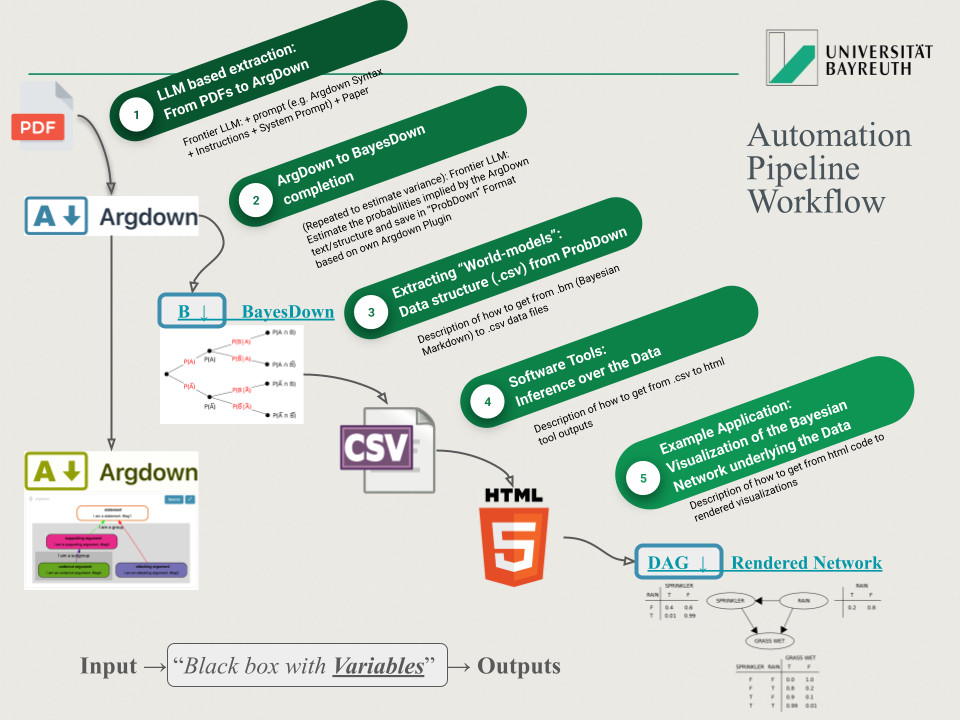
\includegraphics[width=1\linewidth,height=\textheight,keepaspectratio]{images/pipeline.png}}

}

\caption[Five-step AMTAIR automation pipeline from PDFs to Bayesian
networks]{\label{fig-automation_pipeline}AMTAIR Automation Pipeline from
CITATION}

\end{figure}%

\section{Thesis Structure and Roadmap}\label{sec-roadmap}

\textbf{Logical Progression from Theory to Application:}

\begin{itemize}
\tightlist
\item
  \textbf{Context \& Background}: Establish theoretical foundations
  (Bayesian networks, argument mapping) and methodological approach
  (two-stage extraction)
\item
  \textbf{AMTAIR Implementation}: Demonstrate technical feasibility
  through working prototype with validated examples
\item
  \textbf{Critical Analysis}: Examine limitations, failure modes, and
  governance implications through systematic red-teaming
\item
  \textbf{Future Directions}: Connect to broader coordination challenges
  and research agenda
\end{itemize}

\texttt{Each\ section\ builds\ toward\ a\ practical\ implementation\ of\ the\ framework\ while\ maintaining\ both\ theoretical\ rigor\ and\ policy\ relevance,\ demonstrating\ how\ computational\ approaches\ can\ enhance\ rather\ than\ replace\ human\ judgment\ in\ AI\ governance.}

The remainder of this thesis develops the multiplicative benefits
framework from theoretical foundations to practical implementation,
following a progression from abstract principles to concrete
applications:

Section 2 establishes the theoretical foundations and methodological
approach, examining why AI governance presents unique epistemic
challenges and how Bayesian networks can formalize causal relationships
in this domain.

Section 3 presents the AMTAIR implementation, detailing the technical
system that transforms qualitative arguments into formal
representations. It demonstrates the approach through two case studies:
the canonical Rain-Sprinkler-Lawn example and the more complex Carlsmith
model of power-seeking AI.

Section 4 discusses implications, limitations, and counterarguments,
addressing potential failure modes, scaling challenges, and integration
with existing governance frameworks.

Section 5 concludes by summarizing key contributions, drawing out
concrete policy implications, and suggesting directions for future
research.

Throughout this progression, I maintain a dual focus on theoretical
sophistication and practical utility. The framework aims not merely to
advance academic understanding of AI risk but to provide actionable
tools for improving coordination in AI governance.

\begin{center}\rule{0.5\linewidth}{0.5pt}\end{center}

\section{Overview / Table of Contents}\label{overview-table-of-contents}

\bookmarksetup{startatroot}

\chapter{Context}\label{context}

\begin{verbatim}
### 20% of Grade: ~ 29% of text ~ 8700 words ~ 20 pages

- demonstrates understanding of all relevant core concepts

- explains why the question/thesis/problem is relevant in student’s own words (supported by quotations)

- situates it within the debate/course material

- reconstructs selected arguments and identifies relevant assumptions

- describes additional relevant material that has been consulted and integrates it with the course material as well as the research question/thesis/problem
\end{verbatim}

\bookmarksetup{startatroot}

\chapter{Context \& Background}\label{sec-context}

\section{Theoretical Foundations}\label{sec-theoretical-foundations}

\subsection{AI Existential Risk: The Carlsmith
Model}\label{sec-carlsmith-model}

\begin{quote}
Carlsmith's ``Is power-seeking AI an existential risk?'' (2021)
represents one of the most structured approaches to assessing the
probability of existential catastrophe from advanced AI. The analysis
decomposes the overall risk into six key premises, each with an explicit
probability estimate.
\end{quote}

\begin{quote}
\textcite{carlsmith2021} provides the canonical structured approach to
AI existential risk assessment
\end{quote}

\textbf{Six-Premise Decomposition:}

\texttt{Carlsmith\ decomposes\ existential\ risk\ into\ a\ probabilistic\ chain\ with\ explicit\ estimates:}

\begin{enumerate}
\def\labelenumi{\arabic{enumi}.}
\tightlist
\item
  \textbf{Premise 1}: Transformative AI development this century (P ≈
  0.80)
\item
  \textbf{Premise 2}: AI systems pursuing objectives in the world (P ≈
  0.95)
\item
  \textbf{Premise 3}: Systems with power-seeking instrumental incentives
  (P ≈ 0.40)
\item
  \textbf{Premise 4}: Sufficient capability for existential threat (P ≈
  0.65)
\item
  \textbf{Premise 5}: Misaligned systems despite safety efforts (P ≈
  0.50)
\item
  \textbf{Premise 6}: Catastrophic outcomes from misaligned
  power-seeking (P ≈ 0.65)
\end{enumerate}

\textbf{Composite Risk Calculation}: P(doom) ≈ 0.05 (5\%)
\textasciitilde5\% probability of existential catastrophe

\begin{quote}
This structured approach exemplifies the type of reasoning that AMTAIR
aims to formalize and automate, providing both transparency in
assumptions and modularity for critique and refinement.
\end{quote}

\texttt{Carlsmith\textquotesingle{}s\ model\ exemplifies\ the\ type\ of\ structured\ reasoning\ that\ AMTAIR\ aims\ to\ formalize\ and\ automate}

\subsubsection{Why Carlsmith as Ideal Formalization
Target}\label{sec-carlsmith-ideal}

\begin{verbatim}
- Explicitly probabilistic reasoning with quantified estimates
- Clear conditional dependencies between premises  
- Transparent decomposition of complex causal pathways
- Well-documented argumentation available for extraction validation
- Policy-relevant implications requiring formal evaluation
\end{verbatim}

\textbf{Formalization Potential:}

\texttt{Carlsmith\textquotesingle{}s\ model\ represents\ "low-hanging\ fruit"\ for\ automated\ formalization\ because\ it\ already\ exhibits\ explicit\ probabilistic\ reasoning\ with\ clear\ conditional\ dependencies.\ Success\ with\ this\ structured\ argument\ validates\ the\ approach\ for\ less\ explicit\ arguments\ throughout\ AI\ safety\ literature.}

\subsection{The Epistemic Challenge of Policy
Evaluation}\label{sec-epistemic-challenge}

\begin{quote}
AI governance policy evaluation faces unique epistemic challenges that
render traditional policy analysis methods insufficient. The domain
combines complex causal chains with limited empirical grounding, deep
uncertainty about future capabilities, divergent stakeholder worldviews,
and few opportunities for experimental testing before deployment.
\end{quote}

`Traditional methods fall short in several ways:

\begin{itemize}
\tightlist
\item
  Cost-benefit analysis struggles with existential outcomes and deep
  uncertainty
\item
  Scenario planning often lacks probabilistic reasoning necessary for
  rigorous evaluation
\item
  Expert elicitation alone fails to formalize interdependencies between
  variables
\item
  Qualitative approaches obscure crucial assumptions that drive
  conclusions`
\end{itemize}

\textbf{Unprecedented Epistemic Environment:}

\begin{quote}
AI governance policy evaluation faces challenges that render traditional
policy analysis methods insufficient: complex causal chains, deep
uncertainty about unprecedented capabilities, divergent stakeholder
worldviews, and limited opportunities for empirical validation.
\end{quote}

\begin{verbatim}
Specific challenges include:

• **Deep Uncertainty**: Many decisions involve unprecedented scenarios without historical frequency data
• **Complex Causality**: Policy effects propagate through multi-level dependencies (technical → institutional → strategic)
• **Multidisciplinary Integration**: Combining technical facts, ethical principles, and strategic considerations
• **Value-Laden Assessment**: Risk evaluation inherently involves normative judgments about acceptable outcomes
\end{verbatim}

\subsubsection{Unique Difficulties in AI
Governance}\label{sec-unique-difficulties}

\textbf{Complex Causal Chains}: Multi-level dependencies between
technical capabilities, institutional responses, and strategic outcomes

\textbf{Deep Uncertainty}: Unprecedented AI capabilities make historical
analogies insufficient

\begin{quote}
\textcite{lempert2003} on robust decision-making under deep uncertainty
\end{quote}

\textbf{Divergent Worldviews}: Fundamental disagreements about:

\begin{itemize}
\tightlist
\item
  Timeline expectations for transformative AI
\item
  Difficulty of alignment problems
\item
  Effectiveness of governance interventions
\item
  International coordination possibilities
\end{itemize}

\subsubsection{Limitations of Traditional Policy
Analysis}\label{sec-traditional-limitations}

\begin{itemize}
\tightlist
\item
  \textbf{Cost-Benefit Analysis}: Struggles with existential outcomes
  and infinite expected values
\item
  \textbf{Scenario Planning}: Lacks probabilistic reasoning and
  uncertainty quantification
\item
  \textbf{Expert Elicitation}: Fails to formalize complex
  interdependencies between variables
\item
  \textbf{Qualitative Frameworks}: Obscure crucial assumptions and
  parameter sensitivities
\end{itemize}

\textbf{Limitations of Traditional Approaches:}

\begin{itemize}
\tightlist
\item
  \textbf{Cost-Benefit Analysis}: Struggles with existential outcomes
  and infinite expected values
\item
  \textbf{Scenario Planning}: Often lacks probabilistic reasoning
  necessary for rigorous uncertainty quantification
\item
  \textbf{Expert Elicitation}: Fails to formalize complex
  interdependencies between variables and assumptions
\item
  \textbf{Qualitative Frameworks}: Obscure crucial assumptions and
  parameter sensitivities driving conclusions
\end{itemize}

\begin{quote}
\textcite{lempert2003} on robust decision-making under deep uncertainty
provides methodological foundations, but application to AI governance
requires novel integration of argument mapping with probabilistic
modeling.
\end{quote}

\subsection{Argument Mapping and Formal
Representations}\label{sec-argument-mapping}

\begin{quote}
Argument mapping offers a bridge between informal reasoning in natural
language and the formal representations needed for rigorous analysis. By
explicitly identifying claims, premises, inferential relationships, and
support/attack patterns, argument maps make implicit reasoning
structures visible for examination and critique.
\end{quote}

\texttt{The\ progression\ from\ natural\ language\ arguments\ to\ formal\ Bayesian\ networks\ requires\ an\ intermediate\ representation\ that\ preserves\ narrative\ structure\ while\ adding\ mathematical\ precision.\ The\ ArgDown\ format\ serves\ this\ purpose\ by\ encoding\ hierarchical\ relationships\ between\ statements,\ while\ its\ extension,\ BayesDown,\ adds\ probabilistic\ metadata\ to\ enable\ full\ Bayesian\ network\ construction.}

\begin{verbatim}
[Effect_Node]: Description of effect. {"instantiations": ["effect_TRUE", "effect_FALSE"]}
 + [Cause_Node]: Description of direct cause. {"instantiations": ["cause_TRUE", "cause_FALSE"]}
   + [Root_Cause]: Description of indirect cause. {"instantiations": ["root_TRUE", "root_FALSE"]}
\end{verbatim}

\subsection{Bayesian Networks as Knowledge
Representation}\label{sec-bayesian-networks}

\begin{quote}
Bayesian networks provide a formal mathematical framework for
representing causal relationships and reasoning under uncertainty. These
directed acyclic graphs (DAGs) combine qualitative structure---nodes
representing variables and edges representing dependencies---with
quantitative parameters in the form of conditional probability tables.
\end{quote}

`Key properties that make Bayesian networks particularly suited to AI
risk modeling include:

\begin{itemize}
\tightlist
\item
  Natural representation of causal relationships between variables
\item
  Explicit handling of uncertainty through probability distributions
\item
  Support for evidence updating through Bayesian inference
\item
  Capability for interventional reasoning through do-calculus
\item
  Balance between mathematical rigor and intuitive visual
  representation`
\end{itemize}

\begin{figure}

\centering{

\href{https://claude.ai/chat/ab8988f3-18b7-45a5-8a50-b25aa4b34cbf}{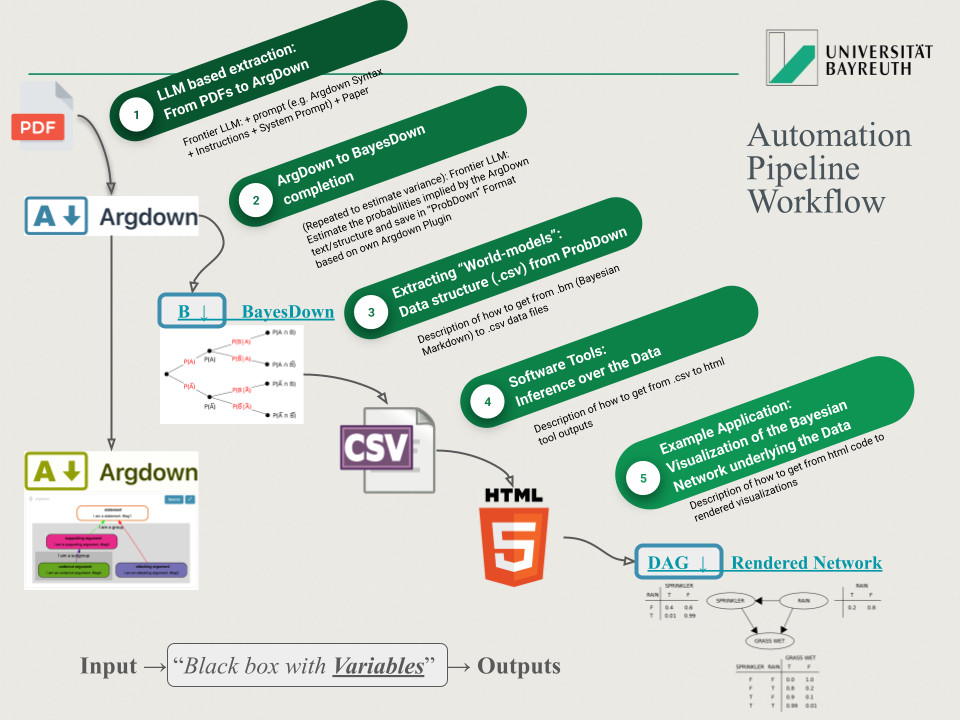
\includegraphics[width=0.7\linewidth,height=\textheight,keepaspectratio]{images/pipeline.png}}

}

\caption{\label{fig-bayesian-network}Example Bayesian Network}

\end{figure}%

\subsubsection{Mathematical
Foundations}\label{sec-mathematical-foundations}

\texttt{Bayesian\ networks\ provide\ a\ formal\ mathematical\ framework\ for\ representing\ causal\ relationships\ and\ reasoning\ under\ uncertainty\ through\ Directed\ Acyclic\ Graphs\ (DAGs)\ combining\ qualitative\ structure\ with\ quantitative\ parameters.}

\textbf{Directed Acyclic Graphs (DAGs)}:

\textbf{Core Components:}

\begin{itemize}
\tightlist
\item
  \textbf{Nodes}: Variables with discrete states representing
  propositions or factors
\item
  \textbf{Edges}: Directed relationships representing conditional
  dependencies
\item
  \textbf{Acyclicity}: Ensuring coherent probabilistic interpretation
  without circular dependencies
\end{itemize}

BNs:

\begin{itemize}
\tightlist
\item
  \textbf{Conditional Probability Tables}: Quantifying
  P(Node\textbar Parents) for all parent state combinations
\end{itemize}

\textbf{Probability Factorization}:
\(P(X_1, X_2, ..., X_n) = \prod_{i=1}^{n} P(X_i | Parents(X_i))\)

\subsubsection{The Rain-Sprinkler-Grass
Example}\label{sec-rain-sprinkler-example}

\textbf{The Rain-Sprinkler-Grass Canonical Example:}

\texttt{This\ simple\ example\ demonstrates\ all\ key\ concepts\ while\ remaining\ intuitive}

\textbf{Network Structure}:

\begin{itemize}
\tightlist
\item
  \textbf{Rain} (root cause): P(rain) = 0.2
\item
  \textbf{Sprinkler} (intermediate): P(sprinkler\textbar rain) varies by
  rain state
\item
  \textbf{Grass\_Wet} (effect): P(wet\textbar rain, sprinkler) depends
  on both causes
\end{itemize}

\textbf{Inference Capabilities}:

\begin{itemize}
\item
  Marginal probabilities: P(grass\_wet) = ?
\item
  Conditional queries: P(rain\textbar grass\_wet) = ?
\item
  Counterfactual analysis: P(grass\_wet\textbar do(sprinkler=false)) = ?
\item
  Marginal probabilities: P(grass\_wet) computed from joint distribution
\item
  Conditional queries: P(rain\textbar grass\_wet) for diagnostic
  reasoning
\item
  Counterfactual analysis: P(grass\_wet\textbar do(sprinkler=false)) for
  intervention effects
\end{itemize}

\begin{verbatim}
python
# Basic network representation
nodes = ['Rain', 'Sprinkler', 'Grass_Wet']
edges = [('Rain', 'Sprinkler'), ('Rain', 'Grass_Wet'), ('Sprinkler', 'Grass_Wet')]

# Conditional probability specification
P_wet_given_causes = {
    (True, True): 0.99,    # Rain=T, Sprinkler=T
    (True, False): 0.80,   # Rain=T, Sprinkler=F  
    (False, True): 0.90,   # Rain=F, Sprinkler=T
    (False, False): 0.01   # Rain=F, Sprinkler=F
}
\end{verbatim}

\subsubsection{Advantages for AI Risk
Modeling}\label{sec-modeling-advantages}

\begin{itemize}
\tightlist
\item
  \textbf{Explicit Uncertainty}: All beliefs represented with
  probability distributions rather than point estimates
\item
  \textbf{Causal Reasoning}: Native support for intervention analysis
  and counterfactual reasoning through do-calculus
\item
  \textbf{Evidence Integration}: Bayesian updating enables principled
  incorporation of new information
\item
  \textbf{Modular Structure}: Complex arguments decomposed into
  manageable, verifiable components
\item
  \textbf{Visual Communication}: Graphical representation facilitates
  understanding across expertise levels
\end{itemize}

\subsection{Argument Mapping and Formal
Representations}\label{sec-argument-mapping}

\subsubsection{From Natural Language to Formal
Models}\label{sec-natural-to-formal}

\textbf{The Representation Challenge}: How to preserve narrative
richness while enabling mathematical analysis

\texttt{The\ core\ methodological\ challenge\ involves\ preserving\ narrative\ richness\ of\ natural\ language\ arguments\ while\ enabling\ mathematical\ analysis—bridging\ interpretive\ reasoning\ favored\ in\ philosophy\ with\ quantitative\ prediction\ favored\ in\ technical\ fields.}

\textbf{ArgDown Syntax}:

\begin{verbatim}
[Conclusion]: Description of the conclusion.
 + [Premise1]: Supporting evidence or reasoning.
   + [Sub-premise]: More detailed supporting factor.
 + [Premise2]: Additional independent support.
\end{verbatim}

\texttt{ArgDown\ uses\ hierarchical\ indentation\ to\ capture\ support/attack\ relationships\ between\ statements,\ making\ argument\ structure\ explicit\ while\ remaining\ human-readable.}

\subsubsection{BayesDown: The Critical
Innovation}\label{sec-bayesdown-innovation}

\texttt{BayesDown\ extends\ ArgDown\ with\ probabilistic\ metadata,\ creating\ a\ hybrid\ format\ that\ bridges\ natural\ language\ and\ mathematical\ modeling:}

\begin{verbatim}
json
{
  "instantiations": ["conclusion_TRUE", "conclusion_FALSE"],
  "priors": {"p(conclusion_TRUE)": "0.7", "p(conclusion_FALSE)": "0.3"},
  "posteriors": {
    "p(conclusion_TRUE|premise1_TRUE,premise2_TRUE)": "0.9",
    "p(conclusion_TRUE|premise1_TRUE,premise2_FALSE)": "0.6",
    "p(conclusion_TRUE|premise1_FALSE,premise2_TRUE)": "0.4",
    "p(conclusion_TRUE|premise1_FALSE,premise2_FALSE)": "0.1"
  }
}
\end{verbatim}

\textbf{Design Principles}:

\begin{itemize}
\tightlist
\item
  \textbf{Human Readable}: Preserves natural language explanations
\item
  \textbf{Machine Processable}: Structured for automated analysis
\item
  \textbf{Probabilistically Complete}: Contains all information for
  Bayesian network construction
\item
  \textbf{Extensible}: Supports additional metadata as needed
\end{itemize}

\subsection{The MTAIR Framework: Achievements and
Limitations}\label{sec-mtair-framework}

\begin{quote}
\textcite{bucknall2022} on the original Modeling Transformative AI Risks
project demonstrates both the value and limitations of manual formal
modeling approaches.
\end{quote}

\begin{quote}
The Modeling Transformative AI Risks (MTAIR) project demonstrated the
value of formal probabilistic modeling for AI safety, but also revealed
significant limitations in the manual approach. While MTAIR successfully
translated complex arguments into Bayesian networks and enabled
sensitivity analysis, the intensive human labor required for model
creation limited both scalability and timeliness.
\end{quote}

\subsubsection{MTAIR's Innovations}\label{sec-mtair-innovations}

\begin{quote}
\textcite{bucknall2022} on the original Modeling Transformative AI Risks
project
\end{quote}

\begin{itemize}
\tightlist
\item
  \textbf{Structured Uncertainty Representation}: Explicit probability
  distributions over key variables
\item
  \textbf{Expert Judgment Integration}: Systematic methods for
  aggregating diverse opinions
\item
  \textbf{Sensitivity Analysis}: Identification of critical
  uncertainties driving outcomes
\item
  \textbf{Policy Application}: Connection between technical models and
  governance implications
\end{itemize}

\textbf{MTAIR's Key Innovations:}

\begin{itemize}
\tightlist
\item
  \textbf{Structured Uncertainty Representation}: Explicit probability
  distributions over key variables rather than point estimates
\item
  \textbf{Expert Judgment Integration}: Systematic methods for
  aggregating diverse expert opinions and beliefs
\item
  \textbf{Sensitivity Analysis}: Identification of critical
  uncertainties that most significantly drive overall conclusions
\item
  \textbf{Policy Application}: Direct connection between technical risk
  models and governance implications
\end{itemize}

`MTAIR's key innovations included:

\begin{itemize}
\tightlist
\item
  Explicit representation of uncertainty through probability
  distributions
\item
  Structured decomposition of complex risk scenarios
\item
  Integration of diverse expert judgments
\item
  Sensitivity analysis to identify critical parameters
\end{itemize}

\subsubsection{Fundamental Limitations Motivating
AMTAIR}\label{sec-mtair-limitations}

\textbf{Scalability Bottleneck}: Manual model construction requires
weeks of expert effort per model

\textbf{Static Models}: No mechanisms for updating as new research
emerges

\textbf{Limited Accessibility}: Technical complexity restricts usage to
specialists

\textbf{Single Worldview Focus}: Difficulty representing multiple
perspectives simultaneously

\texttt{These\ limitations\ create\ the\ opportunity\ for\ automated\ approaches\ that\ can\ scale\ formal\ modeling\ to\ match\ the\ pace\ of\ AI\ governance\ discourse}

\textbf{Fundamental Limitations Motivating AMTAIR:}

\begin{verbatim}
Critical constraints of manual approaches:

• **Scalability Bottleneck**: Manual model construction requires weeks of expert effort per argument
• **Static Nature**: No mechanisms for updating models as new research and evidence emerges  
• **Limited Accessibility**: Technical complexity restricts usage to specialists with formal modeling expertise
• **Single Worldview Focus**: Difficulty representing multiple conflicting perspectives simultaneously
\end{verbatim}

\texttt{These\ limitations\ create\ a\ clear\ opportunity\ for\ automated\ approaches\ that\ can\ scale\ formal\ modeling\ to\ match\ the\ pace\ and\ diversity\ of\ AI\ governance\ discourse.}

Its limitations motivated the current automated approach:

\begin{itemize}
\tightlist
\item
  Manual labor intensity limiting scalability
\item
  Static nature of models once constructed
\item
  Limited accessibility for non-technical stakeholders
\item
  Challenges in representing multiple worldviews simultaneously`
\end{itemize}

\subsection{``A Narrow Path'': Conditional Policy Proposals in
Practice}\label{sec-narrow-path}

\begin{quote}
``A Narrow Path'' represents influential example of conditional policy
proposals in AI governance---identifying interventions that could
succeed under specific conditions rather than universal prescriptions.
\end{quote}

\texttt{However,\ these\ conditions\ remain\ implicitly\ defined\ and\ qualitatively\ described,\ limiting\ rigorous\ evaluation\ and\ comparison\ across\ alternative\ approaches.}

\begin{quote}
``A Narrow Path'' represents an influential example of conditional
policy proposals in AI governance---identifying interventions that could
succeed under specific conditions rather than absolute prescriptions.
However, these conditions remain implicitly defined and qualitatively
described, limiting rigorous evaluation.
\end{quote}

`Formal modeling could enhance such proposals by:

\begin{itemize}
\tightlist
\item
  Making conditions explicit and quantifiable
\item
  Clarifying when interventions would be effective
\item
  Identifying which uncertainties most significantly affect outcomes
\item
  Enabling systematic comparison of alternative approaches
\item
  Supporting robust policy development across possible futures`
\end{itemize}

\textbf{Formal Modeling Enhancement Potential:}

\begin{itemize}
\tightlist
\item
  Making conditions explicit and quantifiable rather than implicit
  assumptions
\item
  Clarifying specific circumstances when interventions would be
  effective versus ineffective
\item
  Identifying which uncertainties most significantly affect intervention
  outcomes
\item
  Enabling systematic comparison of alternative policy approaches under
  uncertainty
\item
  Supporting robust policy development that performs well across
  multiple possible futures
\end{itemize}

\section{Methodology}\label{sec-methodology}

\subsection{Research Design Overview}\label{sec-research-design}

\begin{quote}
This research combines theoretical development with practical
implementation, following an iterative approach that moves between
conceptual refinement and technical validation. The methodology
encompasses formal framework development, computational implementation,
extraction quality assessment, and application to real-world AI
governance questions.
\end{quote}

`The research process follows four main phases:

\begin{enumerate}
\def\labelenumi{\arabic{enumi}.}
\tightlist
\item
  Framework development: Creating the theoretical foundations and formal
  representations
\item
  System implementation: Building the computational tools for extraction
  and analysis
\item
  Validation testing: Assessing extraction quality and system
  performance
\item
  Application evaluation: Applying the framework to concrete AI
  governance questions`
\end{enumerate}

\subsubsection{Hybrid Theoretical-Empirical
Approach}\label{sec-hybrid-approach}

\textbf{Four Integrated Components}:

\begin{enumerate}
\def\labelenumi{\arabic{enumi}.}
\tightlist
\item
  \textbf{Theoretical Development}: Formal framework for automated
  worldview extraction
\item
  \textbf{Technical Implementation}: Working prototype demonstrating
  feasibility
\item
  \textbf{Empirical Validation}: Quality assessment against expert
  benchmarks
\item
  \textbf{Policy Application}: Case studies with real governance
  questions
\end{enumerate}

\textbf{Four Primary Components:}

\begin{enumerate}
\def\labelenumi{\arabic{enumi}.}
\tightlist
\item
  \textbf{Theoretical Development}: Formal framework for automated
  worldview extraction and representation
\item
  \textbf{Technical Implementation}: Working prototype demonstrating
  feasibility and validation
\item
  \textbf{Empirical Validation}: Quality assessment against expert
  benchmarks and known ground truth
\item
  \textbf{Policy Application}: Case studies demonstrating practical
  utility for real governance questions
\end{enumerate}

\textbf{Iterative Development Process:}

\begin{verbatim}
Phase 1: Conceptual Framework Development
↓
Phase 2: Prototype Implementation with Simple Validation Examples  
↓
Phase 3: Complex Real-World Case Application and Evaluation
↓
Phase 4: Policy Impact Assessment and Governance Integration
\end{verbatim}

\subsubsection{Iterative Development
Process}\label{sec-iterative-process}

\begin{verbatim}
Phase 1: Conceptual Framework Development
Phase 2: Prototype Implementation with Simple Examples  
Phase 3: Validation with Complex Real-World Cases
Phase 4: Policy Application and Evaluation
\end{verbatim}

\subsection{Formalizing World Models from AI Safety
Literature}\label{sec-formalizing-world-models}

\begin{quote}
The core methodological challenge involves transforming natural language
arguments in AI safety literature into formal causal models with
explicit probability judgments. This extraction process identifies key
variables, causal relationships, and both explicit and implicit
probability estimates through a systematic pipeline.
\end{quote}

`The extraction approach combines:

\begin{itemize}
\tightlist
\item
  Identification of key variables and entities in text
\item
  Recognition of causal claims and relationships
\item
  Detection of explicit and implicit probability judgments
\item
  Transformation into structured intermediate representations
\item
  Conversion to formal Bayesian networks
\end{itemize}

Large language models facilitate this process through:

\begin{itemize}
\tightlist
\item
  Two-stage prompting that separates structure from probability
  extraction
\item
  Specialized templates for different types of source documents
\item
  Techniques for identifying implicit assumptions and relationships
\item
  Mechanisms for handling ambiguity and uncertainty`
\end{itemize}

\subsection{From Natural Language to Computational
Models}\label{sec-natural-to-computational}

\textbf{The Two-Stage Extraction Architecture:}

\texttt{AMTAIR\ employs\ a\ novel\ two-stage\ process\ that\ separates\ structural\ argument\ extraction\ from\ probability\ quantification,\ enabling\ modular\ improvement\ and\ human\ oversight\ at\ critical\ decision\ points.}

\subsubsection{The Two-Stage Extraction
Process}\label{sec-two-stage-extraction}

\textbf{Stage 1: Structural Extraction (ArgDown)}

\begin{itemize}
\tightlist
\item
  Identify key variables and causal claims
\item
  Extract hierarchical argument structure
\item
  Map logical relationships between elements
\item
  Generate intermediate representation preserving narrative
\end{itemize}

\textbf{Stage 1: Structural Extraction (ArgDown Generation)}

\begin{itemize}
\tightlist
\item
  \textbf{Variable and Claim Identification}: Extract key propositions
  and entities from natural language text
\item
  \textbf{Causal Relationship Mapping}: Identify support/attack
  relationships and conditional dependencies
\item
  \textbf{Hierarchical Structure Construction}: Generate properly nested
  argument representations preserving logical flow
\item
  \textbf{Intermediate Representation}: Create ArgDown format suitable
  for human review and machine processing
\end{itemize}

\begin{Shaded}
\begin{Highlighting}[]
\KeywordTok{def}\NormalTok{ extract\_argument\_structure(text):}
    \CommentTok{"""Extract hierarchical argument structure from natural language"""}
    \CommentTok{\# LLM{-}based extraction with specialized prompts}
\NormalTok{    prompt }\OperatorTok{=}\NormalTok{ ArgumentExtractionPrompt(}
\NormalTok{        text}\OperatorTok{=}\NormalTok{text,}
\NormalTok{        output\_format}\OperatorTok{=}\StringTok{"ArgDown"}\NormalTok{,}
\NormalTok{        focus\_areas}\OperatorTok{=}\NormalTok{[}\StringTok{"causal\_claims"}\NormalTok{, }\StringTok{"probability\_statements"}\NormalTok{, }\StringTok{"conditional\_reasoning"}\NormalTok{]}
\NormalTok{    )}
    
\NormalTok{    structure }\OperatorTok{=}\NormalTok{ llm.complete(prompt)}
    \ControlFlowTok{return}\NormalTok{ validate\_argdown\_syntax(structure)}
\end{Highlighting}
\end{Shaded}

\textbf{Stage 2: Probability Integration (BayesDown)}

\begin{itemize}
\tightlist
\item
  Extract explicit probability statements
\item
  Generate questions for implicit judgments
\item
  Quantify uncertainty and conditional dependencies
\item
  Create complete probabilistic specification
\end{itemize}

\textbf{Stage 2: Probability Integration (BayesDown Enhancement)}

\begin{itemize}
\tightlist
\item
  \textbf{Explicit Probability Extraction}: Identify and parse numerical
  probability statements in source text
\item
  \textbf{Question Generation}: Create systematic elicitation questions
  for implicit probability judgments
\item
  \textbf{Expert Input Integration}: Incorporate domain expertise for
  ambiguous or missing quantifications
\item
  \textbf{Consistency Validation}: Ensure probability assignments
  satisfy basic coherence requirements
\end{itemize}

\begin{Shaded}
\begin{Highlighting}[]
\KeywordTok{def}\NormalTok{ integrate\_probabilities(argdown\_structure, probability\_sources):}
    \CommentTok{"""Convert ArgDown to BayesDown with probabilistic information"""}
\NormalTok{    questions }\OperatorTok{=}\NormalTok{ generate\_probability\_questions(argdown\_structure)}
\NormalTok{    probabilities }\OperatorTok{=}\NormalTok{ extract\_probabilities(probability\_sources, questions)}
    
\NormalTok{    bayesdown }\OperatorTok{=}\NormalTok{ enhance\_with\_probabilities(argdown\_structure, probabilities)}
    \ControlFlowTok{return}\NormalTok{ validate\_probability\_coherence(bayesdown)}
\end{Highlighting}
\end{Shaded}

\subsubsection{LLM Integration Strategy}\label{sec-llm-integration}

\textbf{Prompt Engineering Approach}:

\begin{itemize}
\tightlist
\item
  Specialized prompts for argument structure identification
\item
  Two-stage prompting to separate structure from quantification
\item
  Validation mechanisms to ensure extraction quality
\item
  Iterative refinement based on expert feedback
\end{itemize}

\textbf{Current Capabilities and Limitations}:

\begin{quote}
Frontier LLMs show promising extraction quality but require careful
validation
\end{quote}

\textbf{LLM Integration Strategy:}

\begin{quote}
Frontier language models enable automated extraction but require careful
prompt engineering and validation mechanisms to ensure extraction
quality and consistency.
\end{quote}

\begin{itemize}
\tightlist
\item
  \textbf{Specialized Prompting}: Domain-specific templates for argument
  structure identification
\item
  \textbf{Two-Stage Separation}: Structural and probabilistic extraction
  handled independently for quality control
\item
  \textbf{Validation Mechanisms}: Automated and human review processes
  for extraction accuracy
\item
  \textbf{Iterative Refinement}: Feedback loops enabling continuous
  improvement based on expert assessment
\end{itemize}

\subsection{Directed Acyclic Graphs: Structure and
Semantics}\label{sec-dag-structure}

\begin{quote}
Directed Acyclic Graphs (DAGs) form the mathematical foundation of
Bayesian networks, encoding both the qualitative structure of causal
relationships and the quantitative parameters that define conditional
dependencies. In AI risk modeling, these structures represent causal
pathways to potential outcomes of interest.
\end{quote}

`Key mathematical properties include:

\begin{itemize}
\tightlist
\item
  Acyclicity, ensuring no feedback loops
\item
  Path properties defining information flow
\item
  D-separation criteria determining conditional independence
\item
  Markov blanket defining minimal contextual information
\end{itemize}

\subsubsection{Formal Properties}\label{sec-formal-properties}

\textbf{Acyclicity Requirement}: Ensures coherent probabilistic
interpretation

\textbf{D-Separation}: Conditional independence relationships between
variables

\textbf{Markov Condition}: Each variable independent of non-descendants
given parents

\textbf{Formal Properties Essential for AI Risk Modeling:}

\begin{itemize}
\tightlist
\item
  \textbf{Acyclicity Requirement}: Ensures coherent probabilistic
  interpretation without logical contradictions
\item
  \textbf{D-Separation}: Defines conditional independence relationships
  between variables based on graph structure
\item
  \textbf{Markov Condition}: Each variable conditionally independent of
  non-descendants given parents
\item
  \textbf{Path Analysis}: Causal pathways and information flow through
  the network structure
\end{itemize}

\textbf{Causal Interpretation in AI Governance Context:}

\begin{quote}
\textcite{pearl2009} on causal inference and intervention analysis
provides mathematical foundations for policy evaluation through
do-calculus.
\end{quote}

\begin{itemize}
\tightlist
\item
  \textbf{Edges as Causal Relations}: Directed arrows represent direct
  causal influence between factors
\item
  \textbf{Intervention Analysis}: Do-calculus enables rigorous
  evaluation of policy intervention effects
\item
  \textbf{Counterfactual Reasoning}: ``What if'' scenarios essential for
  governance planning under uncertainty
\item
  \textbf{Evidence Integration}: Bayesian updating for incorporating new
  information and expert judgment
\end{itemize}

\subsubsection{Causal Interpretation}\label{sec-causal-interpretation}

\begin{quote}
\textcite{pearl2009} on causal inference and intervention analysis
\end{quote}

\begin{itemize}
\tightlist
\item
  \textbf{Edges as Causal Relations}: Directed arrows represent direct
  causal influence
\item
  \textbf{Intervention Analysis}: Do-calculus for policy evaluation
\item
  \textbf{Counterfactual Reasoning}: ``What if'' scenarios for
  governance planning
\end{itemize}

Semantic interpretation in AI risk contexts:

\begin{itemize}
\tightlist
\item
  Nodes represent key variables in risk pathways
\item
  Edges represent causal or inferential relationships
\item
  Path blocking corresponds to intervention points
\item
  Probability flows represent risk propagation through systems`
\end{itemize}

\subsection{Quantification of Probabilistic
Judgments}\label{sec-quantification}

\textbf{Linguistic Probability Mapping:}

\texttt{Transforming\ qualitative\ uncertainty\ expressions\ into\ quantitative\ probabilities\ requires\ systematic\ interpretation\ frameworks\ that\ account\ for\ individual\ and\ cultural\ variation.}

\begin{verbatim}
Standard linguistic mappings (with significant individual variation):
• "Very likely" → 0.8-0.9
• "Probable" → 0.6-0.8  
• "Uncertain" → 0.4-0.6
• "Unlikely" → 0.2-0.4
• "Highly improbable" → 0.05-0.15
\end{verbatim}

\begin{quote}
Transforming qualitative judgments in AI safety literature into
quantitative probabilities requires a systematic approach to
interpretation, extraction, and validation. This process combines direct
extraction of explicit numerical statements with inference of implicit
probability judgments from qualitative language.
\end{quote}

`Quantification methods include:

\begin{itemize}
\tightlist
\item
  Direct extraction of explicit numerical statements
\item
  Linguistic mapping of qualitative expressions
\item
  Expert elicitation techniques for ambiguous cases
\item
  Bayesian updating from multiple sources
\end{itemize}

Special challenges in AI risk quantification:

\begin{itemize}
\tightlist
\item
  Deep uncertainty about unprecedented events
\item
  Diverse disciplinary languages and conventions
\item
  Limited empirical basis for calibration
\item
  Value-laden aspects of risk assessment`
\end{itemize}

\subsubsection{From Qualitative to
Quantitative}\label{sec-qualitative-to-quantitative}

\textbf{Linguistic Probability Expressions}:

\begin{itemize}
\tightlist
\item
  ``Very likely'' → 0.8-0.9
\item
  ``Uncertain'' → 0.4-0.6
\item
  ``Highly improbable'' → 0.05-0.15
\end{itemize}

\textbf{Calibration Challenges}:

\begin{itemize}
\tightlist
\item
  Individual variation in linguistic interpretation
\item
  Domain-specific probability anchoring
\item
  Cultural and contextual influences on uncertainty expression
\end{itemize}

\textbf{Calibration and Validation Challenges:}

\begin{itemize}
\tightlist
\item
  Individual variation in linguistic interpretation and probability
  anchoring
\item
  Domain-specific probability anchoring and reference class selection
\item
  Cultural and contextual influences on uncertainty expression and
  tolerance
\item
  Limited empirical basis for calibration in unprecedented scenarios
  like transformative AI
\end{itemize}

\subsubsection{Expert Elicitation Methods}\label{sec-expert-elicitation}

\begin{verbatim}
Direct Probability Assessment: "What is P(outcome)?"
Comparative Assessment: "Is A more likely than B?"  
Frequency Format: "In 100 similar cases, how many would result in outcome?"
Betting Odds: "What odds would you accept for this bet?"
\end{verbatim}

\textbf{Expert Elicitation Methodologies:}

\begin{itemize}
\tightlist
\item
  \textbf{Direct Probability Assessment}: ``What is P(outcome)?'' with
  calibration training
\item
  \textbf{Comparative Assessment}: ``Is A more likely than B?'' for
  relative judgment validation
\item
  \textbf{Frequency Format}: ``In 100 similar cases, how many would
  result in outcome?'' for clearer mental models
\item
  \textbf{Betting Odds}: ``What odds would you accept for this bet?''
  for revealed preference elicitation
\end{itemize}

\subsection{Inference Techniques for Complex
Networks}\label{sec-inference-techniques}

\begin{quote}
Once Bayesian networks are constructed, probabilistic inference enables
reasoning about uncertainties, counterfactuals, and policy
interventions. For the complex networks representing AI risks,
computational approaches must balance accuracy with tractability.
\end{quote}

`Inference methods implemented include:

\begin{itemize}
\tightlist
\item
  Exact methods for smaller networks (variable elimination, junction
  trees)
\item
  Approximate methods for larger networks (Monte Carlo sampling)
\item
  Specialized approaches for rare events
\item
  Intervention modeling for policy evaluation
\end{itemize}

Implementation considerations include:

\begin{itemize}
\tightlist
\item
  Computational complexity management
\item
  Sampling efficiency optimization
\item
  Approximation quality monitoring
\item
  Uncertainty representation in outputs`
\end{itemize}

\subsection{Integration with Prediction Markets and Forecasting
Platforms}\label{sec-prediction-markets}

\begin{quote}
To maintain relevance in a rapidly evolving field, formal models must
integrate with live data sources such as prediction markets and
forecasting platforms. This integration enables continuous updating of
model parameters as new information emerges.
\end{quote}

`Integration approaches include:

\begin{itemize}
\tightlist
\item
  API connections to platforms like Metaculus
\item
  Semantic mapping between forecast questions and model variables
\item
  Weighting mechanisms based on forecaster track records
\item
  Update procedures for incorporating new predictions
\item
  Feedback loops identifying valuable forecast questions
\end{itemize}

Technical implementation involves:

\begin{itemize}
\tightlist
\item
  Standardized data formats across platforms
\item
  Conflict resolution for contradictory sources
\item
  Temporal alignment of forecasts
\item
  Confidence-weighted aggregation methods`
\end{itemize}

\textbf{Live Data Sources for Dynamic Model Updating:}

\begin{itemize}
\tightlist
\item
  \textbf{Metaculus}: Long-term AI predictions and technological
  forecasting
\item
  \textbf{Good Judgment Open}: Geopolitical events and policy outcomes
\item
  \textbf{Manifold Markets}: Diverse question types with rapid market
  response
\item
  \textbf{Internal Expert Forecasting}: Organization-specific
  predictions and assessments
\end{itemize}

\textbf{Data Processing and Integration Pipeline:}

\begin{verbatim}
python
def integrate_forecast_data(model_variables, forecast_platforms):
    """Connect Bayesian network variables to live forecasting data"""
    mappings = create_semantic_mappings(model_variables, forecast_platforms)
    
    for variable, forecasts in mappings.items():
        weighted_forecast = aggregate_forecasts(
            forecasts, 
            weights=calculate_track_record_weights(forecasts)
        )
        model.update_prior(variable, weighted_forecast)
    
    return model.recompute_posteriors()
\end{verbatim}

\textbf{Technical Implementation Challenges:}

\begin{itemize}
\tightlist
\item
  \textbf{Question Mapping}: Connecting forecast questions to specific
  model variables with semantic accuracy
\item
  \textbf{Temporal Alignment}: Handling different forecast horizons and
  update frequencies across platforms
\item
  \textbf{Conflict Resolution}: Principled aggregation when sources
  provide contradictory information
\item
  \textbf{Track Record Weighting}: Incorporating forecaster calibration
  and expertise into aggregation weights
\end{itemize}

\subsubsection{Live Data Sources}\label{sec-live-data}

\textbf{Forecasting Platforms}:

\begin{itemize}
\tightlist
\item
  Metaculus for long-term AI predictions
\item
  Good Judgment Open for geopolitical events
\item
  Manifold Markets for diverse question types
\item
  Internal expert forecasting within organizations
\end{itemize}

\subsubsection{Data Processing Pipeline}\label{sec-data-processing}

\textbf{Question Mapping}: Connecting forecast questions to model
variables

\textbf{Temporal Alignment}: Handling different forecast horizons and
update frequencies

\textbf{Aggregation Methods}: Weighting sources by track record and
relevance

\begin{figure}

\centering{

\href{https://github.com/VJMeyer/submission}{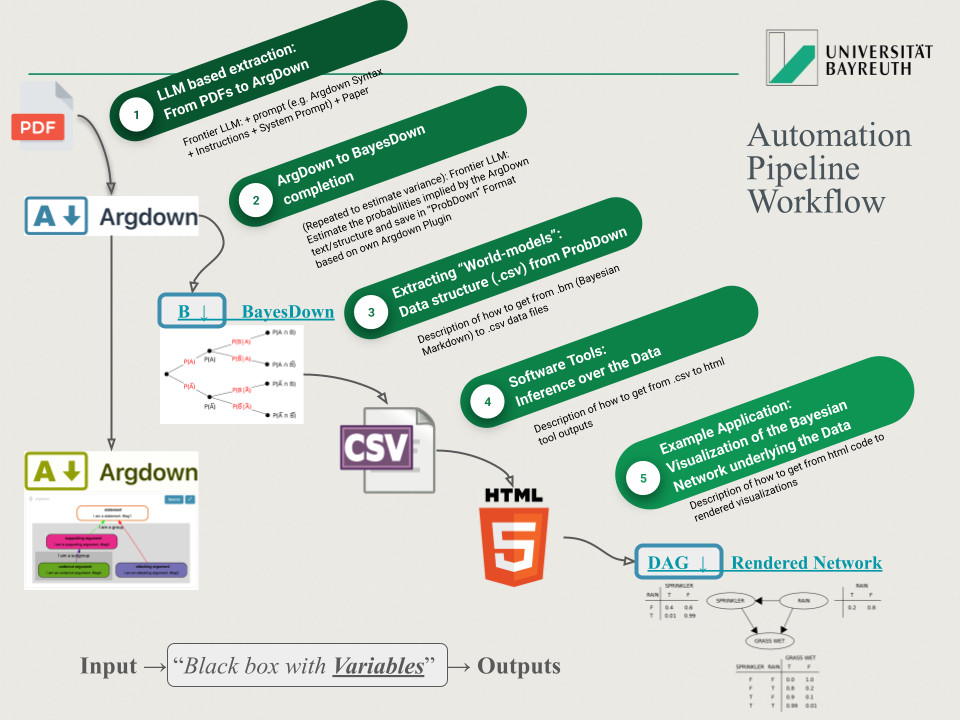
\includegraphics[width=1\linewidth,height=\textheight,keepaspectratio]{images/pipeline.png}}

}

\caption[Five-step AMTAIR automation pipeline from PDFs to Bayesian
networks]{\label{fig-automation_pipeline}AMTAIR Automation Pipeline from
CITATION}

\end{figure}%

Testing crossreferencing grapics Figure~\ref{fig-automation_pipeline}.

\bookmarksetup{startatroot}

\chapter*{Frontmatter}\label{frontmatter}
\addcontentsline{toc}{chapter}{Frontmatter}

\markboth{Frontmatter}{Frontmatter}

\subsection*{\texorpdfstring{\textbf{Acknowledgments}}{Acknowledgments}}\label{acknowledgments}
\addcontentsline{toc}{subsection}{\textbf{Acknowledgments}}

\begin{itemize}
\tightlist
\item
  Academic supervisor (Prof.~Timo Speith) and institution (University of
  Bayreuth)\\
\item
  Research collaborators, especially those connected to the original
  MTAIR project\\
\item
  Technical advisors who provided feedback on implementation aspects\\
\item
  Funding sources and those who provided computational resources or API
  access\\
\item
  Personal supporters who enabled the research through encouragement and
  feedback
\end{itemize}

\bookmarksetup{startatroot}

\chapter*{Prefatory Apparatus: Illustrations and Terminology --- Quick
References}\label{prefatory-apparatus-illustrations-and-terminology-quick-references}
\addcontentsline{toc}{chapter}{Prefatory Apparatus: Illustrations and
Terminology --- Quick References}

\markboth{Prefatory Apparatus: Illustrations and Terminology --- Quick
References}{Prefatory Apparatus: Illustrations and Terminology --- Quick
References}

\section*{List of Tables}\label{list-of-tables}
\addcontentsline{toc}{section}{List of Tables}

\markright{List of Tables}

Table 1: Table name

Table 2: Table name

Table 3: Table name

\begin{itemize}
\tightlist
\item
  Figure 1.1: The coordination crisis in AI governance - visualization
  of fragmentation\\
\item
  Figure 2.1: The Carlsmith model - DAG representation\\
\item
  Figure 3.1: Research design overview - workflow diagram\\
\item
  Figure 3.2: From natural language to BayesDown - transformation
  process\\
\item
  Figure 4.1: ARPA system architecture - component diagram\\
\item
  Figure 4.2: Visualization of Rain-Sprinkler-Grass\_Wet Bayesian
  network - screenshot\\
\item
  Figure 5.1: Extraction quality metrics - comparative chart\\
\item
  Figure 5.2: Comparative analysis of AI governance worldviews - network
  visualization\\
\item
  Table 2.1: Comparison of approaches to AI risk modeling\\
\item
  Table 3.1: Probabilistic translation guide for qualitative
  expressions\\
\item
  Table 4.1: System component responsibilities and interactions\\
\item
  Table 5.1: Policy impact evaluation results - summary metrics
\end{itemize}

\section*{List of Graphics \& Figures}\label{list-of-graphics-figures}
\addcontentsline{toc}{section}{List of Graphics \& Figures}

\markright{List of Graphics \& Figures}

\section*{List of Abbreviations}\label{list-of-abbreviations}
\addcontentsline{toc}{section}{List of Abbreviations}

\markright{List of Abbreviations}

esp.~especially

f., ff.~following

incl.~including

p., pp.~page(s)

MAD Mutually Assured Destruction

\begin{itemize}
\tightlist
\item
  AI - Artificial Intelligence\\
\item
  AGI - Artificial General Intelligence\\
\item
  ARPA - AI Risk Pathway Analyzer\\
\item
  DAG - Directed Acyclic Graph\\
\item
  LLM - Large Language Model\\
\item
  MTAIR - Modeling Transformative AI Risks\\
\item
  P(Doom) - Probability of existential catastrophe from misaligned AI\\
\item
  CPT - Conditional Probability Table
\end{itemize}

\section*{Glossary}\label{glossary}

\markright{Glossary}

\begin{itemize}
\tightlist
\item
  \textbf{Argument mapping}: A method for visually representing the
  structure of arguments\\
\item
  \textbf{BayesDown}: An extension of ArgDown that incorporates
  probabilistic information\\
\item
  \textbf{Bayesian network}: A probabilistic graphical model
  representing variables and their dependencies\\
\item
  \textbf{Conditional probability}: The probability of an event given
  that another event has occurred\\
\item
  \textbf{Directed Acyclic Graph (DAG)}: A graph with directed edges and
  no cycles\\
\item
  \textbf{Existential risk}: Risk of permanent curtailment of humanity's
  potential\\
\item
  \textbf{Power-seeking AI}: AI systems with instrumental incentives to
  acquire resources and power\\
\item
  \textbf{Prediction market}: A market where participants trade
  contracts that resolve based on future events\\
\item
  \textbf{d-separation}: A criterion for identifying conditional
  independence relationships in Bayesian networks\\
\item
  \textbf{Monte Carlo sampling}: A computational technique using random
  sampling to obtain numerical results
\end{itemize}

\section*{\texorpdfstring{Checklists }{Checklists }}\label{checklists}
\addcontentsline{toc}{section}{Checklists }

\markright{Checklists }

\section*{``Usual paper requirements''}\label{usual-paper-requirements}
\addcontentsline{toc}{section}{``Usual paper requirements''}

\markright{``Usual paper requirements''}

\begin{itemize}
\tightlist
\item
  introduce all terminology

  \begin{itemize}
  \tightlist
  \item
    go through text, make sure all terms are defined, explained (and
    added to the list of Abbr.) when first mentioned\\
  \end{itemize}
\item
  readership is intelligent and interested but has no prior knowledge
\end{itemize}

\section*{}\label{section}
\addcontentsline{toc}{section}{}

\markright{}

\section*{(Format:) \textasciitilde{} Anything that makes it easier to
understand}\label{format-anything-that-makes-it-easier-to-understand}
\addcontentsline{toc}{section}{(Format:) \textasciitilde{} Anything that
makes it easier to understand}

\markright{(Format:) \textasciitilde{} Anything that makes it easier to
understand}

\begin{itemize}
\tightlist
\item
  short sentences\\
\item
  paragraphs (one idea per paragraph)\\
\item
  simplicity\\
\item
  !limit use of passive voice!\\
\item
  use active voice, even prefer I over we!\\
\item
  minimise use of ``zombi nouns'' (don't turn verbs/adjectives to
  nouns!)\\
\item
  ``find words that can be cut''
\end{itemize}

-- the paper can \textbf{focus} on \textbf{one aspect of the
presentation}

-- ``open door policy'' for (content) questions

\textasciitilde{} demonstrate ability for novel research

-- ``solve research question with the tools accessible to you''

-- ``show something that has not been shown before / should be
publishable in principle''

-- new idea (or criticism) ``in this field''

-- Outline idea THEN reading with a purpose (answering concrete
questions)

-- ``Only'' confirm that nobody has published the exact same idea on the
same topic

-- pretty much determined by presentation \& proposal but narrow down
further (\& choose supervisor?)

\subsection*{Quarto Features Incompatible with LaTeX
(Below)}\label{quarto-features-incompatible-with-latex-below}

\bookmarksetup{startatroot}

\chapter{Quarto Syntax}\label{quarto-syntax}

\section*{Figures}\label{sec-figues}

\markright{Figures}

\begin{figure}

\centering{

\href{https://github.com/VJMeyer/submission}{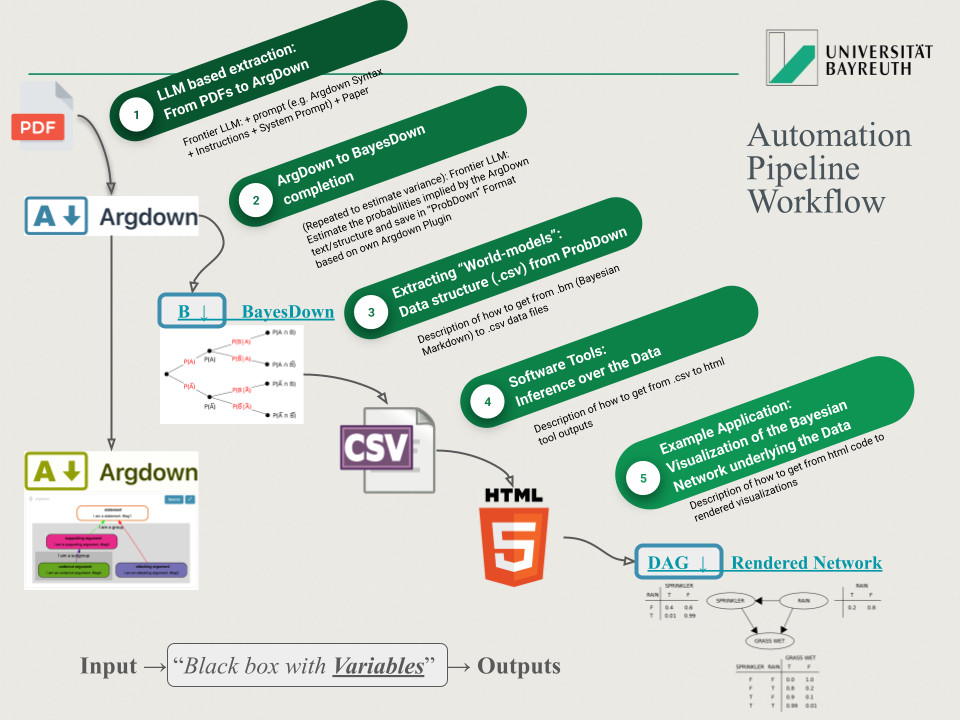
\includegraphics[width=1\linewidth,height=\textheight,keepaspectratio]{images/pipeline.png}}

}

\caption[Five-step AMTAIR automation pipeline from PDFs to Bayesian
networks]{\label{fig-automation_pipeline}AMTAIR Automation Pipeline from
\textcite{bucknall2022}}

\end{figure}%

Testing crossreferencing grapics Figure~\ref{fig-automation_pipeline}.

\begin{figure}


\includegraphics[width=0.3\linewidth,height=\textheight,keepaspectratio]{images/cover.png}

\caption[Short 2 caption]{\label{fig-testgraphic2}Caption/Title 2}

\end{figure}%

Testing crossreferencing grapics Figure~\ref{fig-testgraphic2}.

\section*{Citations}\label{sec-citations}

\markright{Citations}

\textcite{soares2014}

\autocite{soares2014} and \autocite{knuth1984}

Blah Blah \autocites[see][33-35]{knuth1984}[also][chap.~1]{growiec2024}

Blah Blah \autocite[33-35, 38-39 and passim]{knuth1984}

Blah Blah \autocite{growiec2024,knuth1984}.

Growiec says blah \autocite*{growiec2024}

\section{Headings \& Potential Headings}\label{sec-heading}

\texttt{verbatim\ code\ formatting\ for\ notes\ and\ ideas\ to\ be\ included\ (here)}

\begin{verbatim}
Also code blocks for more extensive notes and ideas to be included and checklists
- test 1. 
- test 2. 
- test 3.
2. second
3. third
\end{verbatim}

\begin{quote}
Blockquote formatting for ``Suggested Citations (e.g.~carlsmith 2024 on
\ldots)'' and/or claims which require a citation (e.g.~claim x should be
backed-up by a ciation from the literature)
\end{quote}

Here is an inline note.\footnote{Inlines notes are easier to write,
  since you don't have to pick an identifier and move down to type the
  note.}

Here is a footnote reference,\footnote{Here is the footnote.}

\renewcommand*{\labelitemi}{\textgreater}

Here's some raw inline HTML:

page 1

\newpage{}

page 2

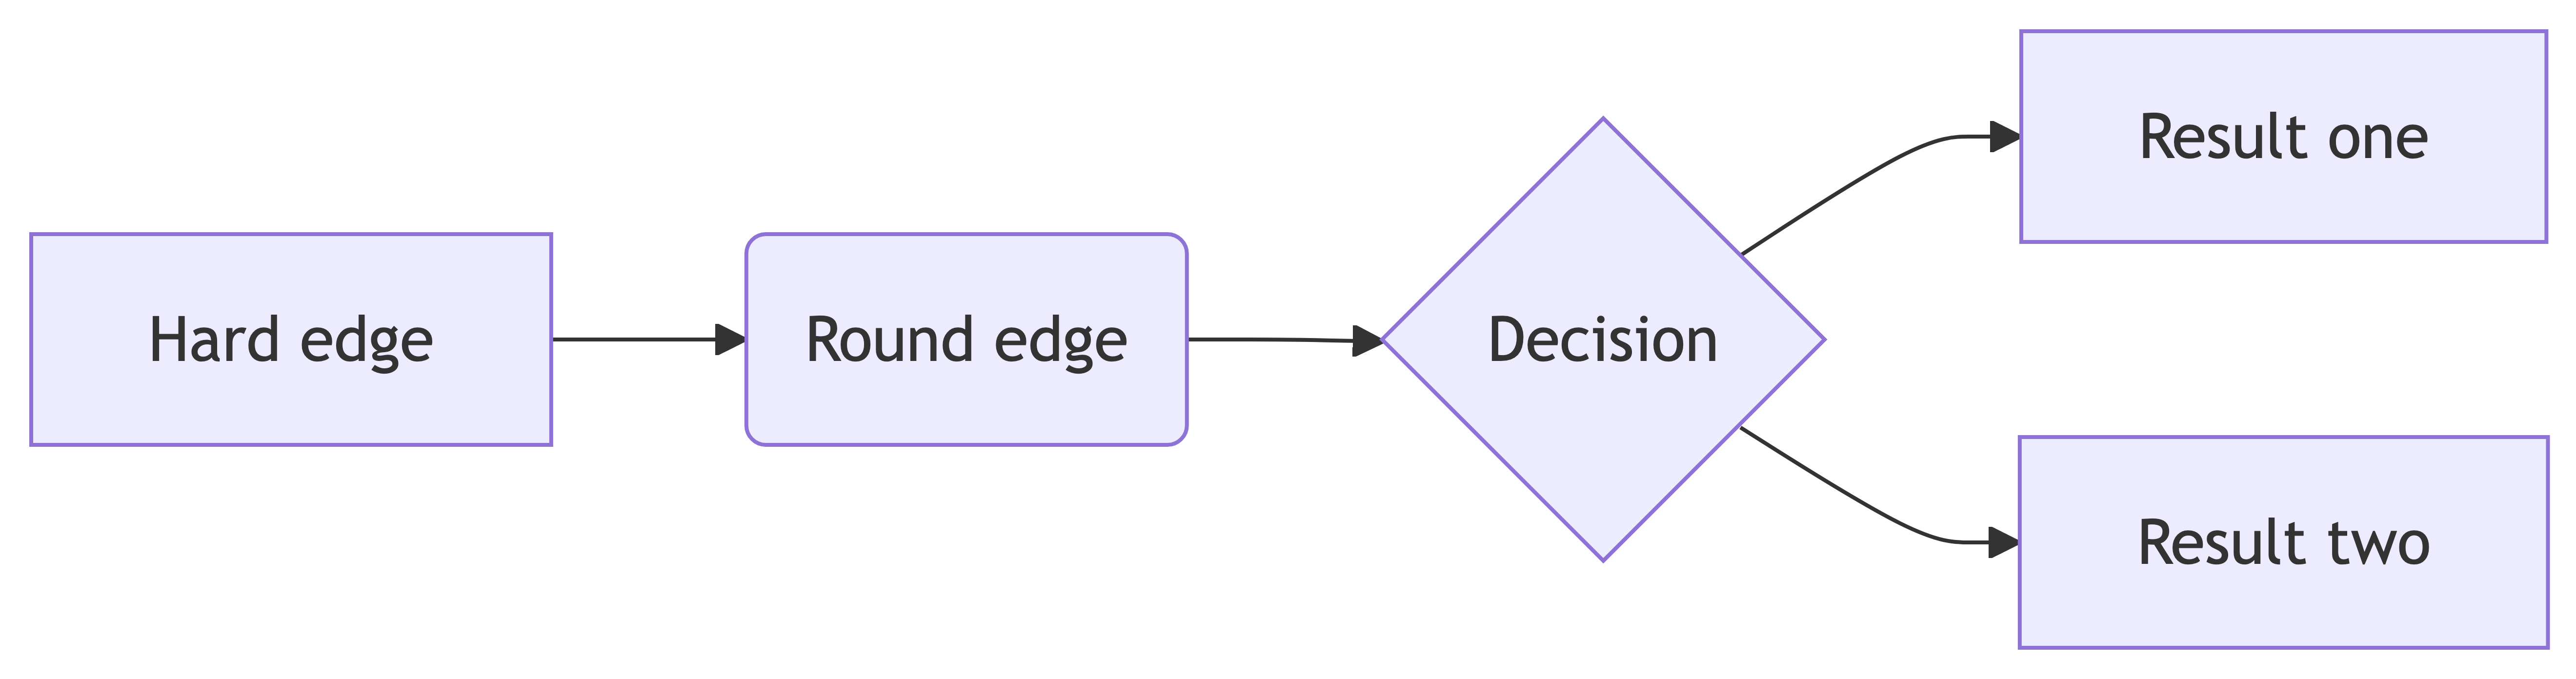
\includegraphics[width=6.88in,height=1.81in]{ref/references_files/figure-latex/mermaid-figure-1.png}

Testing crossreferencing grapics Figure~\ref{fig-automation_pipeline}.

\bookmarksetup{startatroot}

\chapter*{Bibliography (References)}\label{bibliography-references}
\addcontentsline{toc}{chapter}{Bibliography (References)}

\markboth{Bibliography (References)}{Bibliography (References)}

\printbibliography[heading=none]


% Add LOT if requested

% List of figures - explicitly added
\listoffigures

% % Bibliography
% \bibliography{bibliography}
% \bibliographystyle{apalike}


% Add affidavit at the end but still within document environment

\clearpage
\thispagestyle{empty} % Removes page numbering for current page

\newpage


% Top header with logo (left) and department (right)
\begin{minipage}{0.3\textwidth}
  
\includegraphics[width=5cm]{latex/uni-bayreuth-logo.png}
\end{minipage}
\hfill
\begin{minipage}{0.9\textwidth}
  \begin{center}
    -- P\&E Master's Programme --\\
    Chair of Philosophy, Computer\\
    Science \& Artificial Intelligence
  \end{center}
\end{minipage}

% Horizontal rule
\vspace{1.5cm}
\hrule
\vspace{2.5cm}

% Title in bold

  \LARGE\textbf{Affidavit}
\vspace{1.5cm}

\center

\normalsize

% \part*{Affidavit}

    \subsection*{\Large Declaration of Academic Honesty}
	    \vspace{1cm}\noindent \\
	    Hereby, I attest that I have composed and written the presented thesis 
        \vspace*{0.5cm}\noindent \\
        \textit{ \textbf{ Automating the Modelling of Transformative Artificial Intelligence Risks }}
        \vspace*{0.5cm}\noindent \\
        independently on my own, without the use of other than the stated aids and without any other resources than the ones indicated. All thoughts taken directly or indirectly from external sources are properly denoted as such.
	    \vspace{\baselineskip}
	    \\  This paper has neither been previously submitted in the same or a similar form to another authority nor has it been published yet.
	    \vspace{2cm}
	    
    \flushright
    \begin{minipage}{0.5\textwidth}
        \begin{flushleft} \large
        \textsc{Bayreuth}                     %   Place
        on the \\ % 26th of May 2025     \\
        \today           %   Date
        \vspace{2cm}\\
    	{\rule[-3pt]{\linewidth}{.4pt}\par\smallskip  
        \textsc{Valentin Meyer}	\\         %   Your name
    	}
        \end{flushleft}
        \end{minipage}


\end{document}






% Prior versions of template below












% % Main template for University of Bayreuth thesis
% \documentclass[12pt,a4paper]{report}      %   vs book

% % Import custom packages and settings
% 

% % Set page geometry
% \usepackage[a4paper,margin=2.5cm]{geometry}
% \usepackage{graphicx}
% \usepackage{booktabs}
% \usepackage{bookmark}
% \usepackage{hyperref}
% %\usepackage(tocbibind)

% % Define custom commands for metadata
% \newcommand{\subtitle}{}
% \newcommand{\supervisorname}{Supervisor Name}
% \newcommand{\fieldofstudy}{}
% \newcommand{\matriculationnumber}{}
% \newcommand{\submissiondate}{}
% \newcommand{\wordcount}{}
% \providecommand{\tightlist}{%
%   \setlength{\itemsep}{0pt}\setlength{\parskip}{0pt}}

% % Standard document begins
% \begin{document}

% % Create custom title page
% \begin{titlepage}
\thispagestyle{empty}% Remove page number from title page

% Top header with logo (left) and department (right)
\begin{minipage}{0.3\textwidth}
  
\includegraphics[width=5cm]{latex/uni-bayreuth-logo.png}
\end{minipage}
\hfill
\begin{minipage}{0.9\textwidth}
  \begin{center}
    -- P\&E Master's Programme --\\
    Chair of Philosophy, Computer\\
    Science \& Artificial Intelligence
  \end{center}
\end{minipage}

% Horizontal rule
\vspace{1.5cm}
\hrule
\vspace{2cm}

% Title in bold
\begin{center}
  \Large\textbf{Automating the Modelling of
Transformative Artificial Intelligence Risks}
\end{center}
\vspace{0.2cm}

\begin{center}
  -----
\end{center}
\vspace{0.2cm}

% Subtitle in italics with quotation marks
\begin{center}
  \normalsize``\textit{An Epistemic Framework for Leveraging Frontier AI Systems
to Upscale Conditional Policy Assessments in Bayesian Networks on a Narrow Path towards Existencial Safety }''
\end{center}
\vspace{0.2cm}

\begin{center}
  -----
\end{center}
\vspace{0.2cm}

% Thesis designation
\begin{center}
  A thesis submitted at the Department of Philosophy\\[0.4cm]
  for the degree of \textit{Master of Arts in Philosophy \& Economics}
\end{center}

\vspace{1.5cm}
% Horizontal rule
\hrule
\vspace{1.5cm}

% Author and supervisor information with precise alignment
\begin{minipage}[t]{0.48\textwidth}
  \textbf{Author:}\\[0.3cm]
  \href{https://www.vjmeyer.org}{Valentin Jakob Meyer}\\
  \href{mailto:Valentin.meyer@uni-bayreuth.de}{Valentin.meyer@uni-bayreuth.de}\\
  \textit{Matriculation Number:} 1828610\\
  \textit{Tel.:} +49 (1573) 4512494\\
  Pielmühler Straße 15\\
  52066 Lappersdorf
\end{minipage}
\hfill
\begin{minipage}[t]{0.48\textwidth}
  \begin{flushright}
    \textbf{Supervisor:}\\[0.3cm]
    \href{mailto:timo.speith@uni-bayreuth.de}{Dr. Timo Speith}\\[0.3cm]
    \textit{Word Count:}\\
    30.000\\[0.15cm]
    \textit{Source / Identifier:}\\
    \href{https://github.com/VJMeyer/submission}{Document URL}
  \end{flushright}
\end{minipage}

% Date at bottom
\vfill
\begin{center}
  26th of May 2025
\end{center}
\end{titlepage}

% % \pagenumbering{arabic} % Switch to Arabic page numbering
% % \setcounter{page}{1} % Reset page numbers to 1

% % Rest of document
% % \listoffigures
% % \input{\listoffigures}

% \bookmarksetup{startatroot}

\chapter*{Preface}\label{preface}
\addcontentsline{toc}{chapter}{Preface}

\markboth{Preface}{Preface}

This is a Quarto book.

To learn more about Quarto books visit
\url{https://quarto.org/docs/books}.

\bookmarksetup{startatroot}

\chapter*{Abstract}\label{sec-Abstract}
\addcontentsline{toc}{chapter}{Abstract}

\markboth{Abstract}{Abstract}

\bookmarksetup{startatroot}

\chapter*{Outline(s): Table of Contents}\label{sec-ToC}
\addcontentsline{toc}{chapter}{Outline(s): Table of Contents}

\markboth{Outline(s): Table of Contents}{Outline(s): Table of Contents}

\bookmarksetup{startatroot}

\chapter{Introduction}\label{introduction}

\begin{quote}
Subtitle: An Epistemic Framework for Leveraging Frontier AI Systems to
Upscale Conditional Policy Assessments in Bayesian Networks on a Narrow
Path towards Existential Safety
\end{quote}

\begin{verbatim}
### 10% of Grade: ~ 14% of text ~ 4200 words ~ 10 pages

-   introduces and motivates the core question or problem

-   provides context for discussion (places issue within a larger debate or sphere of relevance)

-   states precise thesis or position the author will argue for

-   provides roadmap indicating structure and key content points of the essay
\end{verbatim}

\section*{Abstract}\label{sec-abstract}
\addcontentsline{toc}{section}{Abstract}

\markright{Abstract}

\begin{quote}
The coordination crisis in AI governance presents a paradoxical
challenge: unprecedented investment in AI safety coexists alongside
fundamental coordination failures across technical, policy, and ethical
domains. These divisions systematically increase existential risk. This
thesis introduces AMTAIR (Automating Transformative AI Risk Modeling), a
computational approach addressing this coordination failure by
automating the extraction of probabilistic world models from AI safety
literature using frontier language models. The system implements an
end-to-end pipeline transforming unstructured text into interactive
Bayesian networks through a novel two-stage extraction process that
bridges communication gaps between stakeholders.
\end{quote}

\texttt{The\ coordination\ crisis\ in\ AI\ governance\ presents\ a\ paradoxical\ challenge:\ unprecedented\ investment\ in\ AI\ safety\ coexists\ alongside\ fundamental\ coordination\ failures\ across\ technical,\ policy,\ and\ ethical\ domains.\ These\ divisions\ systematically\ increase\ existential\ risk\ by\ creating\ safety\ gaps,\ misallocating\ resources,\ and\ fostering\ inconsistent\ approaches\ to\ interdependent\ problems.}

\begin{quote}
This thesis introduces AMTAIR (Automating Transformative AI Risk
Modeling), a computational approach that addresses this coordination
failure by automating the extraction of probabilistic world models from
AI safety literature using frontier language models.
\end{quote}

\texttt{The\ AMTAIR\ system\ implements\ an\ end-to-end\ pipeline\ that\ transforms\ unstructured\ text\ into\ interactive\ Bayesian\ networks\ through\ a\ novel\ two-stage\ extraction\ process:\ first\ capturing\ argument\ structure\ in\ ArgDown\ format,\ then\ enhancing\ it\ with\ probability\ information\ in\ BayesDown.\ This\ approach\ bridges\ communication\ gaps\ between\ stakeholders\ by\ making\ implicit\ models\ explicit,\ enabling\ comparison\ across\ different\ worldviews,\ providing\ a\ common\ language\ for\ discussing\ probabilistic\ relationships,\ and\ supporting\ policy\ evaluation\ across\ diverse\ scenarios.}

\bookmarksetup{startatroot}

\chapter{Introduction}\label{sec-introduction}

\texttt{{[}x{]}\ \ introduces\ and\ motivates\ the\ core\ question\ or\ problem}

\section{The Coordination Crisis in AI
Governance}\label{sec-coordination-crisis}

As AI capabilities advance at an accelerating pace---demonstrated by the
rapid progression from GPT-3 to GPT-4, Claude, and beyond---we face a
governance challenge unlike any in human history: how to ensure
increasingly powerful AI systems remain aligned with human values and
beneficial to humanity's long-term flourishing. This challenge becomes
particularly acute when considering the possibility of transformative AI
systems that could drastically alter civilization's trajectory,
potentially including existential risks from misaligned systems.

\begin{quote}
Despite unprecedented investment in AI safety research, rapidly growing
awareness among key stakeholders, and proliferating frameworks for
responsible AI development, we face what I'll term the ``coordination
crisis'' in AI governance---a systemic failure to align diverse efforts
across technical, policy, and strategic domains into a coherent response
proportionate to the risks we face.
\end{quote}

`The AI governance landscape exhibits a peculiar paradox: extraordinary
activity alongside fundamental coordination failure. Consider the
current state of affairs:

Technical safety researchers develop increasingly sophisticated
alignment techniques, but often without clear implementation pathways to
deployment contexts. Policy specialists craft principles and regulatory
frameworks without sufficient technical grounding to ensure their
practical efficacy. Ethicists articulate normative principles that lack
operational specificity. Strategy researchers identify critical
uncertainties but struggle to translate these into actionable guidance.`

\texttt{Opening\ with\ the\ empirical\ paradox:\ record\ investment\ in\ AI\ safety\ coexisting\ with\ fragmented,\ ineffective\ governance\ responses}

\subsection{Empirical Paradox: Investment Alongside
Fragmentation}\label{sec-empirical-paradox}

\begin{itemize}
\tightlist
\item
  \textbf{The Fragmentation Problem}: Technical researchers, policy
  specialists, and strategic analysts operate with incompatible
  frameworks
\end{itemize}

\subsection{Systematic Risk Increase Through Coordination
Failure}\label{sec-risk-increase}

\begin{itemize}
\tightlist
\item
  \textbf{Systemic Risk Amplification}: How coordination failures
  systematically increase existential risk through safety gaps and
  resource misallocation
\end{itemize}

\subsection{Historical Parallels and Temporal
Urgency}\label{sec-historical-parallels}

\begin{itemize}
\tightlist
\item
  \textbf{The Scaling Challenge}: Traditional governance approaches
  cannot match the pace of capability development
\end{itemize}

\section{Research Question and Scope}\label{sec-research-question}

This thesis addresses a specific dimension of the coordination challenge
by investigating the question: \textbf{Can frontier AI technologies be
utilized to automate the modeling of transformative AI risks, enabling
robust prediction of policy impacts?}

\texttt{This\ thesis\ addresses\ a\ specific\ dimension\ of\ the\ coordination\ challenge\ by\ investigating\ how\ computational\ approaches\ can\ formalize\ the\ worldviews\ and\ arguments\ underlying\ AI\ safety\ discourse,\ transforming\ qualitative\ disagreements\ into\ quantitative\ models\ suitable\ for\ rigorous\ policy\ evaluation.}

To break this down into its components:

\begin{itemize}
\tightlist
\item
  \textbf{Frontier AI Technologies}: Today's most capable language
  models (GPT-4, Claude-3 level systems)
\item
  \textbf{Automated Modeling}: Using these systems to extract and
  formalize argument structures from natural language
\item
  \textbf{Transformative AI Risks}: Potentially catastrophic outcomes
  from advanced AI systems, particularly existential risks
\item
  \textbf{Policy Impact Prediction}: Evaluating how governance
  interventions might alter probability distributions over outcomes
\end{itemize}

\textbf{Central Question}: Can frontier AI technologies be utilized to
automate the modeling of transformative AI risks, enabling robust
prediction of policy impacts?

\texttt{AMTAIR\ represents\ the\ first\ computational\ framework\ for\ automated\ extraction\ and\ formalization\ of\ AI\ governance\ worldviews}

\textbf{Core Innovation}:

\begin{itemize}
\tightlist
\item
  Automated transformation of qualitative governance arguments into
  quantitative Bayesian networks
\item
  Integration of prediction markets with formal models for dynamic risk
  assessment
\item
  Cross-worldview policy evaluation under deep uncertainty
\end{itemize}

\textbf{Scope Boundaries:}

\texttt{The\ investigation\ encompasses\ both\ theoretical\ development\ and\ practical\ implementation,\ focusing\ specifically\ on\ existential\ risks\ from\ misaligned\ AI\ systems\ rather\ than\ broader\ AI\ ethics\ concerns.\ This\ narrowed\ scope\ enables\ deep\ technical\ development\ while\ addressing\ the\ highest-stakes\ coordination\ challenges.}

The scope encompasses both theoretical development and practical
implementation. Theoretically, I develop a framework for representing
diverse perspectives on AI risk in a common formal language.
Practically, I implement this framework in a computational system---the
AI Risk Pathway Analyzer (ARPA)---that enables interactive exploration
of how policy interventions might alter existential risk.

\section{The Multiplicative Benefits
Framework}\label{sec-multiplicative-benefits}

\textbf{Core Innovation:} The combination of three elements---automated
extraction, prediction market integration, and formal policy
evaluation---creates multiplicative rather than additive benefits for AI
governance.

The central thesis of this work is that combining three
elements---automated worldview extraction, prediction market
integration, and formal policy evaluation---creates multiplicative
rather than merely additive benefits for AI governance. Each component
enhances the others, creating a system more valuable than the sum of its
parts.

\textbf{Automated worldview extraction} using frontier language models
addresses the scaling bottleneck in current approaches to AI risk
modeling. The Modeling Transformative AI Risks (MTAIR) project
demonstrated the value of formal representation but required extensive
manual effort to translate qualitative arguments into quantitative
models. Automation enables processing orders of magnitude more content,
incorporating diverse perspectives, and maintaining models in near
real-time as new arguments emerge.

\textbf{Prediction market integration} grounds these models in
collective forecasting intelligence. By connecting formal
representations to live forecasting platforms, the system can
incorporate timely judgments about critical uncertainties from
calibrated forecasters. This creates a dynamic feedback loop, where
models inform forecasters and forecasts update models.

\textbf{Formal policy evaluation} transforms static risk assessments
into actionable guidance by modeling how specific interventions might
alter critical parameters. This enables conditional
forecasting---understanding not just the probability of adverse outcomes
but how those probabilities change under different policy regimes.

\textbf{Synergistic Components:}

\begin{enumerate}
\def\labelenumi{\arabic{enumi}.}
\tightlist
\item
  \textbf{Automated Worldview Extraction}: Scaling formal modeling from
  manual (MTAIR) to automated approaches using frontier LLMs
\item
  \textbf{Live Data Integration}: Connecting models to prediction
  markets and forecasting platforms for dynamic calibration and live
  updating
\item
  \textbf{Policy Evaluation}: Enabling rigorous counterfactual analysis
  of governance interventions across worldviews
\end{enumerate}

\texttt{The\ synergy\ emerges\ because\ automation\ enables\ comprehensive\ data\ integration,\ markets\ inform\ and\ validate\ models,\ and\ evaluation\ gains\ precision\ from\ both\ automated\ extraction\ and\ market-based\ calibration.}

\texttt{The\ combination\ creates\ multiplicative\ rather\ than\ additive\ value—automation\ enables\ comprehensive\ data\ integration,\ markets\ inform\ models,\ evaluation\ gains\ precision\ from\ both}

\begin{figure}

\centering{

\href{https://github.com/VJMeyer/submission}{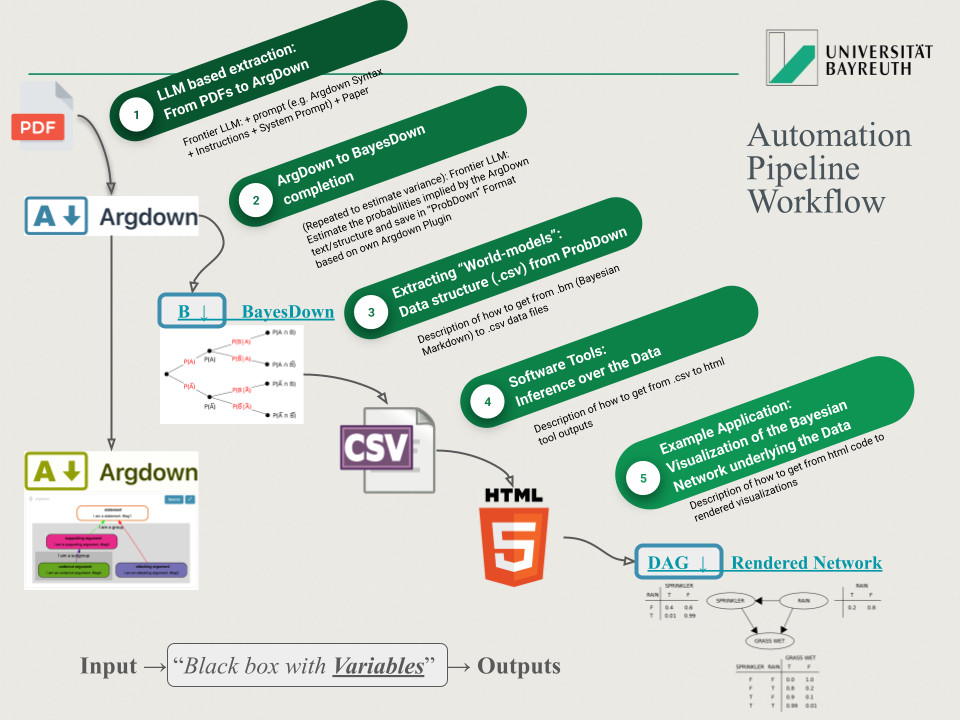
\includegraphics[width=1\linewidth,height=\textheight,keepaspectratio]{images/pipeline.png}}

}

\caption[Five-step AMTAIR automation pipeline from PDFs to Bayesian
networks]{\label{fig-automation_pipeline}AMTAIR Automation Pipeline from
CITATION}

\end{figure}%

\section{Thesis Structure and Roadmap}\label{sec-roadmap}

\textbf{Logical Progression from Theory to Application:}

\begin{itemize}
\tightlist
\item
  \textbf{Context \& Background}: Establish theoretical foundations
  (Bayesian networks, argument mapping) and methodological approach
  (two-stage extraction)
\item
  \textbf{AMTAIR Implementation}: Demonstrate technical feasibility
  through working prototype with validated examples
\item
  \textbf{Critical Analysis}: Examine limitations, failure modes, and
  governance implications through systematic red-teaming
\item
  \textbf{Future Directions}: Connect to broader coordination challenges
  and research agenda
\end{itemize}

\texttt{Each\ section\ builds\ toward\ a\ practical\ implementation\ of\ the\ framework\ while\ maintaining\ both\ theoretical\ rigor\ and\ policy\ relevance,\ demonstrating\ how\ computational\ approaches\ can\ enhance\ rather\ than\ replace\ human\ judgment\ in\ AI\ governance.}

The remainder of this thesis develops the multiplicative benefits
framework from theoretical foundations to practical implementation,
following a progression from abstract principles to concrete
applications:

Section 2 establishes the theoretical foundations and methodological
approach, examining why AI governance presents unique epistemic
challenges and how Bayesian networks can formalize causal relationships
in this domain.

Section 3 presents the AMTAIR implementation, detailing the technical
system that transforms qualitative arguments into formal
representations. It demonstrates the approach through two case studies:
the canonical Rain-Sprinkler-Lawn example and the more complex Carlsmith
model of power-seeking AI.

Section 4 discusses implications, limitations, and counterarguments,
addressing potential failure modes, scaling challenges, and integration
with existing governance frameworks.

Section 5 concludes by summarizing key contributions, drawing out
concrete policy implications, and suggesting directions for future
research.

Throughout this progression, I maintain a dual focus on theoretical
sophistication and practical utility. The framework aims not merely to
advance academic understanding of AI risk but to provide actionable
tools for improving coordination in AI governance.

\begin{center}\rule{0.5\linewidth}{0.5pt}\end{center}

\section{Overview / Table of Contents}\label{overview-table-of-contents}

\bookmarksetup{startatroot}

\chapter{Context}\label{context}

\begin{verbatim}
### 20% of Grade: ~ 29% of text ~ 8700 words ~ 20 pages

- demonstrates understanding of all relevant core concepts

- explains why the question/thesis/problem is relevant in student’s own words (supported by quotations)

- situates it within the debate/course material

- reconstructs selected arguments and identifies relevant assumptions

- describes additional relevant material that has been consulted and integrates it with the course material as well as the research question/thesis/problem
\end{verbatim}

\bookmarksetup{startatroot}

\chapter{Context \& Background}\label{sec-context}

\section{Theoretical Foundations}\label{sec-theoretical-foundations}

\subsection{AI Existential Risk: The Carlsmith
Model}\label{sec-carlsmith-model}

\begin{quote}
Carlsmith's ``Is power-seeking AI an existential risk?'' (2021)
represents one of the most structured approaches to assessing the
probability of existential catastrophe from advanced AI. The analysis
decomposes the overall risk into six key premises, each with an explicit
probability estimate.
\end{quote}

\begin{quote}
\textcite{carlsmith2021} provides the canonical structured approach to
AI existential risk assessment
\end{quote}

\textbf{Six-Premise Decomposition:}

\texttt{Carlsmith\ decomposes\ existential\ risk\ into\ a\ probabilistic\ chain\ with\ explicit\ estimates:}

\begin{enumerate}
\def\labelenumi{\arabic{enumi}.}
\tightlist
\item
  \textbf{Premise 1}: Transformative AI development this century (P ≈
  0.80)
\item
  \textbf{Premise 2}: AI systems pursuing objectives in the world (P ≈
  0.95)
\item
  \textbf{Premise 3}: Systems with power-seeking instrumental incentives
  (P ≈ 0.40)
\item
  \textbf{Premise 4}: Sufficient capability for existential threat (P ≈
  0.65)
\item
  \textbf{Premise 5}: Misaligned systems despite safety efforts (P ≈
  0.50)
\item
  \textbf{Premise 6}: Catastrophic outcomes from misaligned
  power-seeking (P ≈ 0.65)
\end{enumerate}

\textbf{Composite Risk Calculation}: P(doom) ≈ 0.05 (5\%)
\textasciitilde5\% probability of existential catastrophe

\begin{quote}
This structured approach exemplifies the type of reasoning that AMTAIR
aims to formalize and automate, providing both transparency in
assumptions and modularity for critique and refinement.
\end{quote}

\texttt{Carlsmith\textquotesingle{}s\ model\ exemplifies\ the\ type\ of\ structured\ reasoning\ that\ AMTAIR\ aims\ to\ formalize\ and\ automate}

\subsubsection{Why Carlsmith as Ideal Formalization
Target}\label{sec-carlsmith-ideal}

\begin{verbatim}
- Explicitly probabilistic reasoning with quantified estimates
- Clear conditional dependencies between premises  
- Transparent decomposition of complex causal pathways
- Well-documented argumentation available for extraction validation
- Policy-relevant implications requiring formal evaluation
\end{verbatim}

\textbf{Formalization Potential:}

\texttt{Carlsmith\textquotesingle{}s\ model\ represents\ "low-hanging\ fruit"\ for\ automated\ formalization\ because\ it\ already\ exhibits\ explicit\ probabilistic\ reasoning\ with\ clear\ conditional\ dependencies.\ Success\ with\ this\ structured\ argument\ validates\ the\ approach\ for\ less\ explicit\ arguments\ throughout\ AI\ safety\ literature.}

\subsection{The Epistemic Challenge of Policy
Evaluation}\label{sec-epistemic-challenge}

\begin{quote}
AI governance policy evaluation faces unique epistemic challenges that
render traditional policy analysis methods insufficient. The domain
combines complex causal chains with limited empirical grounding, deep
uncertainty about future capabilities, divergent stakeholder worldviews,
and few opportunities for experimental testing before deployment.
\end{quote}

`Traditional methods fall short in several ways:

\begin{itemize}
\tightlist
\item
  Cost-benefit analysis struggles with existential outcomes and deep
  uncertainty
\item
  Scenario planning often lacks probabilistic reasoning necessary for
  rigorous evaluation
\item
  Expert elicitation alone fails to formalize interdependencies between
  variables
\item
  Qualitative approaches obscure crucial assumptions that drive
  conclusions`
\end{itemize}

\textbf{Unprecedented Epistemic Environment:}

\begin{quote}
AI governance policy evaluation faces challenges that render traditional
policy analysis methods insufficient: complex causal chains, deep
uncertainty about unprecedented capabilities, divergent stakeholder
worldviews, and limited opportunities for empirical validation.
\end{quote}

\begin{verbatim}
Specific challenges include:

• **Deep Uncertainty**: Many decisions involve unprecedented scenarios without historical frequency data
• **Complex Causality**: Policy effects propagate through multi-level dependencies (technical → institutional → strategic)
• **Multidisciplinary Integration**: Combining technical facts, ethical principles, and strategic considerations
• **Value-Laden Assessment**: Risk evaluation inherently involves normative judgments about acceptable outcomes
\end{verbatim}

\subsubsection{Unique Difficulties in AI
Governance}\label{sec-unique-difficulties}

\textbf{Complex Causal Chains}: Multi-level dependencies between
technical capabilities, institutional responses, and strategic outcomes

\textbf{Deep Uncertainty}: Unprecedented AI capabilities make historical
analogies insufficient

\begin{quote}
\textcite{lempert2003} on robust decision-making under deep uncertainty
\end{quote}

\textbf{Divergent Worldviews}: Fundamental disagreements about:

\begin{itemize}
\tightlist
\item
  Timeline expectations for transformative AI
\item
  Difficulty of alignment problems
\item
  Effectiveness of governance interventions
\item
  International coordination possibilities
\end{itemize}

\subsubsection{Limitations of Traditional Policy
Analysis}\label{sec-traditional-limitations}

\begin{itemize}
\tightlist
\item
  \textbf{Cost-Benefit Analysis}: Struggles with existential outcomes
  and infinite expected values
\item
  \textbf{Scenario Planning}: Lacks probabilistic reasoning and
  uncertainty quantification
\item
  \textbf{Expert Elicitation}: Fails to formalize complex
  interdependencies between variables
\item
  \textbf{Qualitative Frameworks}: Obscure crucial assumptions and
  parameter sensitivities
\end{itemize}

\textbf{Limitations of Traditional Approaches:}

\begin{itemize}
\tightlist
\item
  \textbf{Cost-Benefit Analysis}: Struggles with existential outcomes
  and infinite expected values
\item
  \textbf{Scenario Planning}: Often lacks probabilistic reasoning
  necessary for rigorous uncertainty quantification
\item
  \textbf{Expert Elicitation}: Fails to formalize complex
  interdependencies between variables and assumptions
\item
  \textbf{Qualitative Frameworks}: Obscure crucial assumptions and
  parameter sensitivities driving conclusions
\end{itemize}

\begin{quote}
\textcite{lempert2003} on robust decision-making under deep uncertainty
provides methodological foundations, but application to AI governance
requires novel integration of argument mapping with probabilistic
modeling.
\end{quote}

\subsection{Argument Mapping and Formal
Representations}\label{sec-argument-mapping}

\begin{quote}
Argument mapping offers a bridge between informal reasoning in natural
language and the formal representations needed for rigorous analysis. By
explicitly identifying claims, premises, inferential relationships, and
support/attack patterns, argument maps make implicit reasoning
structures visible for examination and critique.
\end{quote}

\texttt{The\ progression\ from\ natural\ language\ arguments\ to\ formal\ Bayesian\ networks\ requires\ an\ intermediate\ representation\ that\ preserves\ narrative\ structure\ while\ adding\ mathematical\ precision.\ The\ ArgDown\ format\ serves\ this\ purpose\ by\ encoding\ hierarchical\ relationships\ between\ statements,\ while\ its\ extension,\ BayesDown,\ adds\ probabilistic\ metadata\ to\ enable\ full\ Bayesian\ network\ construction.}

\begin{verbatim}
[Effect_Node]: Description of effect. {"instantiations": ["effect_TRUE", "effect_FALSE"]}
 + [Cause_Node]: Description of direct cause. {"instantiations": ["cause_TRUE", "cause_FALSE"]}
   + [Root_Cause]: Description of indirect cause. {"instantiations": ["root_TRUE", "root_FALSE"]}
\end{verbatim}

\subsection{Bayesian Networks as Knowledge
Representation}\label{sec-bayesian-networks}

\begin{quote}
Bayesian networks provide a formal mathematical framework for
representing causal relationships and reasoning under uncertainty. These
directed acyclic graphs (DAGs) combine qualitative structure---nodes
representing variables and edges representing dependencies---with
quantitative parameters in the form of conditional probability tables.
\end{quote}

`Key properties that make Bayesian networks particularly suited to AI
risk modeling include:

\begin{itemize}
\tightlist
\item
  Natural representation of causal relationships between variables
\item
  Explicit handling of uncertainty through probability distributions
\item
  Support for evidence updating through Bayesian inference
\item
  Capability for interventional reasoning through do-calculus
\item
  Balance between mathematical rigor and intuitive visual
  representation`
\end{itemize}

\begin{figure}

\centering{

\href{https://claude.ai/chat/ab8988f3-18b7-45a5-8a50-b25aa4b34cbf}{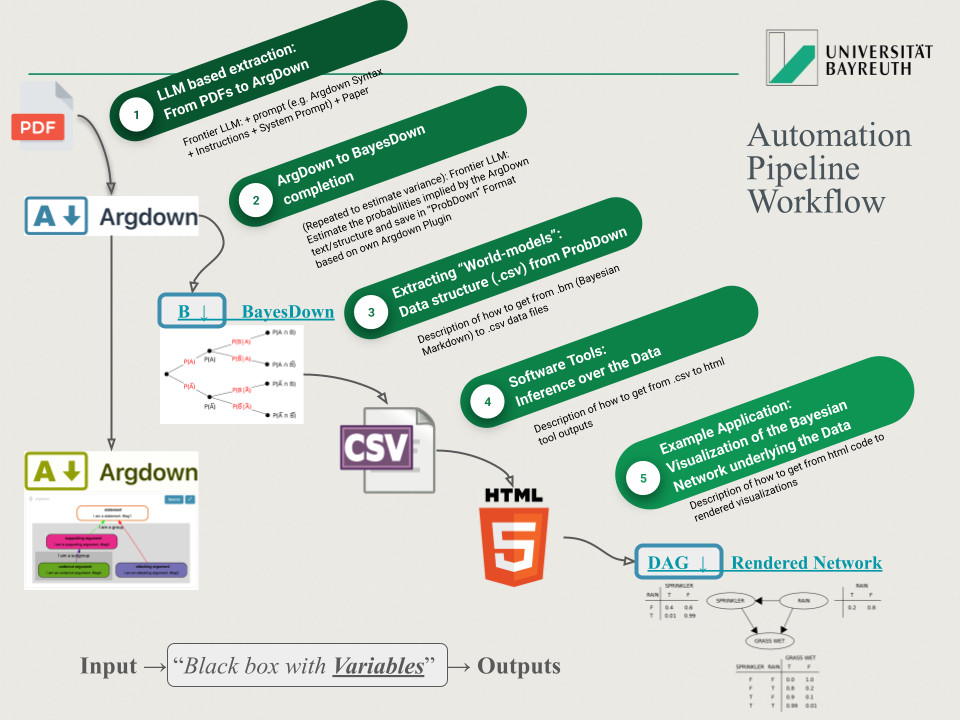
\includegraphics[width=0.7\linewidth,height=\textheight,keepaspectratio]{images/pipeline.png}}

}

\caption{\label{fig-bayesian-network}Example Bayesian Network}

\end{figure}%

\subsubsection{Mathematical
Foundations}\label{sec-mathematical-foundations}

\texttt{Bayesian\ networks\ provide\ a\ formal\ mathematical\ framework\ for\ representing\ causal\ relationships\ and\ reasoning\ under\ uncertainty\ through\ Directed\ Acyclic\ Graphs\ (DAGs)\ combining\ qualitative\ structure\ with\ quantitative\ parameters.}

\textbf{Directed Acyclic Graphs (DAGs)}:

\textbf{Core Components:}

\begin{itemize}
\tightlist
\item
  \textbf{Nodes}: Variables with discrete states representing
  propositions or factors
\item
  \textbf{Edges}: Directed relationships representing conditional
  dependencies
\item
  \textbf{Acyclicity}: Ensuring coherent probabilistic interpretation
  without circular dependencies
\end{itemize}

BNs:

\begin{itemize}
\tightlist
\item
  \textbf{Conditional Probability Tables}: Quantifying
  P(Node\textbar Parents) for all parent state combinations
\end{itemize}

\textbf{Probability Factorization}:
\(P(X_1, X_2, ..., X_n) = \prod_{i=1}^{n} P(X_i | Parents(X_i))\)

\subsubsection{The Rain-Sprinkler-Grass
Example}\label{sec-rain-sprinkler-example}

\textbf{The Rain-Sprinkler-Grass Canonical Example:}

\texttt{This\ simple\ example\ demonstrates\ all\ key\ concepts\ while\ remaining\ intuitive}

\textbf{Network Structure}:

\begin{itemize}
\tightlist
\item
  \textbf{Rain} (root cause): P(rain) = 0.2
\item
  \textbf{Sprinkler} (intermediate): P(sprinkler\textbar rain) varies by
  rain state
\item
  \textbf{Grass\_Wet} (effect): P(wet\textbar rain, sprinkler) depends
  on both causes
\end{itemize}

\textbf{Inference Capabilities}:

\begin{itemize}
\item
  Marginal probabilities: P(grass\_wet) = ?
\item
  Conditional queries: P(rain\textbar grass\_wet) = ?
\item
  Counterfactual analysis: P(grass\_wet\textbar do(sprinkler=false)) = ?
\item
  Marginal probabilities: P(grass\_wet) computed from joint distribution
\item
  Conditional queries: P(rain\textbar grass\_wet) for diagnostic
  reasoning
\item
  Counterfactual analysis: P(grass\_wet\textbar do(sprinkler=false)) for
  intervention effects
\end{itemize}

\begin{verbatim}
python
# Basic network representation
nodes = ['Rain', 'Sprinkler', 'Grass_Wet']
edges = [('Rain', 'Sprinkler'), ('Rain', 'Grass_Wet'), ('Sprinkler', 'Grass_Wet')]

# Conditional probability specification
P_wet_given_causes = {
    (True, True): 0.99,    # Rain=T, Sprinkler=T
    (True, False): 0.80,   # Rain=T, Sprinkler=F  
    (False, True): 0.90,   # Rain=F, Sprinkler=T
    (False, False): 0.01   # Rain=F, Sprinkler=F
}
\end{verbatim}

\subsubsection{Advantages for AI Risk
Modeling}\label{sec-modeling-advantages}

\begin{itemize}
\tightlist
\item
  \textbf{Explicit Uncertainty}: All beliefs represented with
  probability distributions rather than point estimates
\item
  \textbf{Causal Reasoning}: Native support for intervention analysis
  and counterfactual reasoning through do-calculus
\item
  \textbf{Evidence Integration}: Bayesian updating enables principled
  incorporation of new information
\item
  \textbf{Modular Structure}: Complex arguments decomposed into
  manageable, verifiable components
\item
  \textbf{Visual Communication}: Graphical representation facilitates
  understanding across expertise levels
\end{itemize}

\subsection{Argument Mapping and Formal
Representations}\label{sec-argument-mapping}

\subsubsection{From Natural Language to Formal
Models}\label{sec-natural-to-formal}

\textbf{The Representation Challenge}: How to preserve narrative
richness while enabling mathematical analysis

\texttt{The\ core\ methodological\ challenge\ involves\ preserving\ narrative\ richness\ of\ natural\ language\ arguments\ while\ enabling\ mathematical\ analysis—bridging\ interpretive\ reasoning\ favored\ in\ philosophy\ with\ quantitative\ prediction\ favored\ in\ technical\ fields.}

\textbf{ArgDown Syntax}:

\begin{verbatim}
[Conclusion]: Description of the conclusion.
 + [Premise1]: Supporting evidence or reasoning.
   + [Sub-premise]: More detailed supporting factor.
 + [Premise2]: Additional independent support.
\end{verbatim}

\texttt{ArgDown\ uses\ hierarchical\ indentation\ to\ capture\ support/attack\ relationships\ between\ statements,\ making\ argument\ structure\ explicit\ while\ remaining\ human-readable.}

\subsubsection{BayesDown: The Critical
Innovation}\label{sec-bayesdown-innovation}

\texttt{BayesDown\ extends\ ArgDown\ with\ probabilistic\ metadata,\ creating\ a\ hybrid\ format\ that\ bridges\ natural\ language\ and\ mathematical\ modeling:}

\begin{verbatim}
json
{
  "instantiations": ["conclusion_TRUE", "conclusion_FALSE"],
  "priors": {"p(conclusion_TRUE)": "0.7", "p(conclusion_FALSE)": "0.3"},
  "posteriors": {
    "p(conclusion_TRUE|premise1_TRUE,premise2_TRUE)": "0.9",
    "p(conclusion_TRUE|premise1_TRUE,premise2_FALSE)": "0.6",
    "p(conclusion_TRUE|premise1_FALSE,premise2_TRUE)": "0.4",
    "p(conclusion_TRUE|premise1_FALSE,premise2_FALSE)": "0.1"
  }
}
\end{verbatim}

\textbf{Design Principles}:

\begin{itemize}
\tightlist
\item
  \textbf{Human Readable}: Preserves natural language explanations
\item
  \textbf{Machine Processable}: Structured for automated analysis
\item
  \textbf{Probabilistically Complete}: Contains all information for
  Bayesian network construction
\item
  \textbf{Extensible}: Supports additional metadata as needed
\end{itemize}

\subsection{The MTAIR Framework: Achievements and
Limitations}\label{sec-mtair-framework}

\begin{quote}
\textcite{bucknall2022} on the original Modeling Transformative AI Risks
project demonstrates both the value and limitations of manual formal
modeling approaches.
\end{quote}

\begin{quote}
The Modeling Transformative AI Risks (MTAIR) project demonstrated the
value of formal probabilistic modeling for AI safety, but also revealed
significant limitations in the manual approach. While MTAIR successfully
translated complex arguments into Bayesian networks and enabled
sensitivity analysis, the intensive human labor required for model
creation limited both scalability and timeliness.
\end{quote}

\subsubsection{MTAIR's Innovations}\label{sec-mtair-innovations}

\begin{quote}
\textcite{bucknall2022} on the original Modeling Transformative AI Risks
project
\end{quote}

\begin{itemize}
\tightlist
\item
  \textbf{Structured Uncertainty Representation}: Explicit probability
  distributions over key variables
\item
  \textbf{Expert Judgment Integration}: Systematic methods for
  aggregating diverse opinions
\item
  \textbf{Sensitivity Analysis}: Identification of critical
  uncertainties driving outcomes
\item
  \textbf{Policy Application}: Connection between technical models and
  governance implications
\end{itemize}

\textbf{MTAIR's Key Innovations:}

\begin{itemize}
\tightlist
\item
  \textbf{Structured Uncertainty Representation}: Explicit probability
  distributions over key variables rather than point estimates
\item
  \textbf{Expert Judgment Integration}: Systematic methods for
  aggregating diverse expert opinions and beliefs
\item
  \textbf{Sensitivity Analysis}: Identification of critical
  uncertainties that most significantly drive overall conclusions
\item
  \textbf{Policy Application}: Direct connection between technical risk
  models and governance implications
\end{itemize}

`MTAIR's key innovations included:

\begin{itemize}
\tightlist
\item
  Explicit representation of uncertainty through probability
  distributions
\item
  Structured decomposition of complex risk scenarios
\item
  Integration of diverse expert judgments
\item
  Sensitivity analysis to identify critical parameters
\end{itemize}

\subsubsection{Fundamental Limitations Motivating
AMTAIR}\label{sec-mtair-limitations}

\textbf{Scalability Bottleneck}: Manual model construction requires
weeks of expert effort per model

\textbf{Static Models}: No mechanisms for updating as new research
emerges

\textbf{Limited Accessibility}: Technical complexity restricts usage to
specialists

\textbf{Single Worldview Focus}: Difficulty representing multiple
perspectives simultaneously

\texttt{These\ limitations\ create\ the\ opportunity\ for\ automated\ approaches\ that\ can\ scale\ formal\ modeling\ to\ match\ the\ pace\ of\ AI\ governance\ discourse}

\textbf{Fundamental Limitations Motivating AMTAIR:}

\begin{verbatim}
Critical constraints of manual approaches:

• **Scalability Bottleneck**: Manual model construction requires weeks of expert effort per argument
• **Static Nature**: No mechanisms for updating models as new research and evidence emerges  
• **Limited Accessibility**: Technical complexity restricts usage to specialists with formal modeling expertise
• **Single Worldview Focus**: Difficulty representing multiple conflicting perspectives simultaneously
\end{verbatim}

\texttt{These\ limitations\ create\ a\ clear\ opportunity\ for\ automated\ approaches\ that\ can\ scale\ formal\ modeling\ to\ match\ the\ pace\ and\ diversity\ of\ AI\ governance\ discourse.}

Its limitations motivated the current automated approach:

\begin{itemize}
\tightlist
\item
  Manual labor intensity limiting scalability
\item
  Static nature of models once constructed
\item
  Limited accessibility for non-technical stakeholders
\item
  Challenges in representing multiple worldviews simultaneously`
\end{itemize}

\subsection{``A Narrow Path'': Conditional Policy Proposals in
Practice}\label{sec-narrow-path}

\begin{quote}
``A Narrow Path'' represents influential example of conditional policy
proposals in AI governance---identifying interventions that could
succeed under specific conditions rather than universal prescriptions.
\end{quote}

\texttt{However,\ these\ conditions\ remain\ implicitly\ defined\ and\ qualitatively\ described,\ limiting\ rigorous\ evaluation\ and\ comparison\ across\ alternative\ approaches.}

\begin{quote}
``A Narrow Path'' represents an influential example of conditional
policy proposals in AI governance---identifying interventions that could
succeed under specific conditions rather than absolute prescriptions.
However, these conditions remain implicitly defined and qualitatively
described, limiting rigorous evaluation.
\end{quote}

`Formal modeling could enhance such proposals by:

\begin{itemize}
\tightlist
\item
  Making conditions explicit and quantifiable
\item
  Clarifying when interventions would be effective
\item
  Identifying which uncertainties most significantly affect outcomes
\item
  Enabling systematic comparison of alternative approaches
\item
  Supporting robust policy development across possible futures`
\end{itemize}

\textbf{Formal Modeling Enhancement Potential:}

\begin{itemize}
\tightlist
\item
  Making conditions explicit and quantifiable rather than implicit
  assumptions
\item
  Clarifying specific circumstances when interventions would be
  effective versus ineffective
\item
  Identifying which uncertainties most significantly affect intervention
  outcomes
\item
  Enabling systematic comparison of alternative policy approaches under
  uncertainty
\item
  Supporting robust policy development that performs well across
  multiple possible futures
\end{itemize}

\section{Methodology}\label{sec-methodology}

\subsection{Research Design Overview}\label{sec-research-design}

\begin{quote}
This research combines theoretical development with practical
implementation, following an iterative approach that moves between
conceptual refinement and technical validation. The methodology
encompasses formal framework development, computational implementation,
extraction quality assessment, and application to real-world AI
governance questions.
\end{quote}

`The research process follows four main phases:

\begin{enumerate}
\def\labelenumi{\arabic{enumi}.}
\tightlist
\item
  Framework development: Creating the theoretical foundations and formal
  representations
\item
  System implementation: Building the computational tools for extraction
  and analysis
\item
  Validation testing: Assessing extraction quality and system
  performance
\item
  Application evaluation: Applying the framework to concrete AI
  governance questions`
\end{enumerate}

\subsubsection{Hybrid Theoretical-Empirical
Approach}\label{sec-hybrid-approach}

\textbf{Four Integrated Components}:

\begin{enumerate}
\def\labelenumi{\arabic{enumi}.}
\tightlist
\item
  \textbf{Theoretical Development}: Formal framework for automated
  worldview extraction
\item
  \textbf{Technical Implementation}: Working prototype demonstrating
  feasibility
\item
  \textbf{Empirical Validation}: Quality assessment against expert
  benchmarks
\item
  \textbf{Policy Application}: Case studies with real governance
  questions
\end{enumerate}

\textbf{Four Primary Components:}

\begin{enumerate}
\def\labelenumi{\arabic{enumi}.}
\tightlist
\item
  \textbf{Theoretical Development}: Formal framework for automated
  worldview extraction and representation
\item
  \textbf{Technical Implementation}: Working prototype demonstrating
  feasibility and validation
\item
  \textbf{Empirical Validation}: Quality assessment against expert
  benchmarks and known ground truth
\item
  \textbf{Policy Application}: Case studies demonstrating practical
  utility for real governance questions
\end{enumerate}

\textbf{Iterative Development Process:}

\begin{verbatim}
Phase 1: Conceptual Framework Development
↓
Phase 2: Prototype Implementation with Simple Validation Examples  
↓
Phase 3: Complex Real-World Case Application and Evaluation
↓
Phase 4: Policy Impact Assessment and Governance Integration
\end{verbatim}

\subsubsection{Iterative Development
Process}\label{sec-iterative-process}

\begin{verbatim}
Phase 1: Conceptual Framework Development
Phase 2: Prototype Implementation with Simple Examples  
Phase 3: Validation with Complex Real-World Cases
Phase 4: Policy Application and Evaluation
\end{verbatim}

\subsection{Formalizing World Models from AI Safety
Literature}\label{sec-formalizing-world-models}

\begin{quote}
The core methodological challenge involves transforming natural language
arguments in AI safety literature into formal causal models with
explicit probability judgments. This extraction process identifies key
variables, causal relationships, and both explicit and implicit
probability estimates through a systematic pipeline.
\end{quote}

`The extraction approach combines:

\begin{itemize}
\tightlist
\item
  Identification of key variables and entities in text
\item
  Recognition of causal claims and relationships
\item
  Detection of explicit and implicit probability judgments
\item
  Transformation into structured intermediate representations
\item
  Conversion to formal Bayesian networks
\end{itemize}

Large language models facilitate this process through:

\begin{itemize}
\tightlist
\item
  Two-stage prompting that separates structure from probability
  extraction
\item
  Specialized templates for different types of source documents
\item
  Techniques for identifying implicit assumptions and relationships
\item
  Mechanisms for handling ambiguity and uncertainty`
\end{itemize}

\subsection{From Natural Language to Computational
Models}\label{sec-natural-to-computational}

\textbf{The Two-Stage Extraction Architecture:}

\texttt{AMTAIR\ employs\ a\ novel\ two-stage\ process\ that\ separates\ structural\ argument\ extraction\ from\ probability\ quantification,\ enabling\ modular\ improvement\ and\ human\ oversight\ at\ critical\ decision\ points.}

\subsubsection{The Two-Stage Extraction
Process}\label{sec-two-stage-extraction}

\textbf{Stage 1: Structural Extraction (ArgDown)}

\begin{itemize}
\tightlist
\item
  Identify key variables and causal claims
\item
  Extract hierarchical argument structure
\item
  Map logical relationships between elements
\item
  Generate intermediate representation preserving narrative
\end{itemize}

\textbf{Stage 1: Structural Extraction (ArgDown Generation)}

\begin{itemize}
\tightlist
\item
  \textbf{Variable and Claim Identification}: Extract key propositions
  and entities from natural language text
\item
  \textbf{Causal Relationship Mapping}: Identify support/attack
  relationships and conditional dependencies
\item
  \textbf{Hierarchical Structure Construction}: Generate properly nested
  argument representations preserving logical flow
\item
  \textbf{Intermediate Representation}: Create ArgDown format suitable
  for human review and machine processing
\end{itemize}

\begin{Shaded}
\begin{Highlighting}[]
\KeywordTok{def}\NormalTok{ extract\_argument\_structure(text):}
    \CommentTok{"""Extract hierarchical argument structure from natural language"""}
    \CommentTok{\# LLM{-}based extraction with specialized prompts}
\NormalTok{    prompt }\OperatorTok{=}\NormalTok{ ArgumentExtractionPrompt(}
\NormalTok{        text}\OperatorTok{=}\NormalTok{text,}
\NormalTok{        output\_format}\OperatorTok{=}\StringTok{"ArgDown"}\NormalTok{,}
\NormalTok{        focus\_areas}\OperatorTok{=}\NormalTok{[}\StringTok{"causal\_claims"}\NormalTok{, }\StringTok{"probability\_statements"}\NormalTok{, }\StringTok{"conditional\_reasoning"}\NormalTok{]}
\NormalTok{    )}
    
\NormalTok{    structure }\OperatorTok{=}\NormalTok{ llm.complete(prompt)}
    \ControlFlowTok{return}\NormalTok{ validate\_argdown\_syntax(structure)}
\end{Highlighting}
\end{Shaded}

\textbf{Stage 2: Probability Integration (BayesDown)}

\begin{itemize}
\tightlist
\item
  Extract explicit probability statements
\item
  Generate questions for implicit judgments
\item
  Quantify uncertainty and conditional dependencies
\item
  Create complete probabilistic specification
\end{itemize}

\textbf{Stage 2: Probability Integration (BayesDown Enhancement)}

\begin{itemize}
\tightlist
\item
  \textbf{Explicit Probability Extraction}: Identify and parse numerical
  probability statements in source text
\item
  \textbf{Question Generation}: Create systematic elicitation questions
  for implicit probability judgments
\item
  \textbf{Expert Input Integration}: Incorporate domain expertise for
  ambiguous or missing quantifications
\item
  \textbf{Consistency Validation}: Ensure probability assignments
  satisfy basic coherence requirements
\end{itemize}

\begin{Shaded}
\begin{Highlighting}[]
\KeywordTok{def}\NormalTok{ integrate\_probabilities(argdown\_structure, probability\_sources):}
    \CommentTok{"""Convert ArgDown to BayesDown with probabilistic information"""}
\NormalTok{    questions }\OperatorTok{=}\NormalTok{ generate\_probability\_questions(argdown\_structure)}
\NormalTok{    probabilities }\OperatorTok{=}\NormalTok{ extract\_probabilities(probability\_sources, questions)}
    
\NormalTok{    bayesdown }\OperatorTok{=}\NormalTok{ enhance\_with\_probabilities(argdown\_structure, probabilities)}
    \ControlFlowTok{return}\NormalTok{ validate\_probability\_coherence(bayesdown)}
\end{Highlighting}
\end{Shaded}

\subsubsection{LLM Integration Strategy}\label{sec-llm-integration}

\textbf{Prompt Engineering Approach}:

\begin{itemize}
\tightlist
\item
  Specialized prompts for argument structure identification
\item
  Two-stage prompting to separate structure from quantification
\item
  Validation mechanisms to ensure extraction quality
\item
  Iterative refinement based on expert feedback
\end{itemize}

\textbf{Current Capabilities and Limitations}:

\begin{quote}
Frontier LLMs show promising extraction quality but require careful
validation
\end{quote}

\textbf{LLM Integration Strategy:}

\begin{quote}
Frontier language models enable automated extraction but require careful
prompt engineering and validation mechanisms to ensure extraction
quality and consistency.
\end{quote}

\begin{itemize}
\tightlist
\item
  \textbf{Specialized Prompting}: Domain-specific templates for argument
  structure identification
\item
  \textbf{Two-Stage Separation}: Structural and probabilistic extraction
  handled independently for quality control
\item
  \textbf{Validation Mechanisms}: Automated and human review processes
  for extraction accuracy
\item
  \textbf{Iterative Refinement}: Feedback loops enabling continuous
  improvement based on expert assessment
\end{itemize}

\subsection{Directed Acyclic Graphs: Structure and
Semantics}\label{sec-dag-structure}

\begin{quote}
Directed Acyclic Graphs (DAGs) form the mathematical foundation of
Bayesian networks, encoding both the qualitative structure of causal
relationships and the quantitative parameters that define conditional
dependencies. In AI risk modeling, these structures represent causal
pathways to potential outcomes of interest.
\end{quote}

`Key mathematical properties include:

\begin{itemize}
\tightlist
\item
  Acyclicity, ensuring no feedback loops
\item
  Path properties defining information flow
\item
  D-separation criteria determining conditional independence
\item
  Markov blanket defining minimal contextual information
\end{itemize}

\subsubsection{Formal Properties}\label{sec-formal-properties}

\textbf{Acyclicity Requirement}: Ensures coherent probabilistic
interpretation

\textbf{D-Separation}: Conditional independence relationships between
variables

\textbf{Markov Condition}: Each variable independent of non-descendants
given parents

\textbf{Formal Properties Essential for AI Risk Modeling:}

\begin{itemize}
\tightlist
\item
  \textbf{Acyclicity Requirement}: Ensures coherent probabilistic
  interpretation without logical contradictions
\item
  \textbf{D-Separation}: Defines conditional independence relationships
  between variables based on graph structure
\item
  \textbf{Markov Condition}: Each variable conditionally independent of
  non-descendants given parents
\item
  \textbf{Path Analysis}: Causal pathways and information flow through
  the network structure
\end{itemize}

\textbf{Causal Interpretation in AI Governance Context:}

\begin{quote}
\textcite{pearl2009} on causal inference and intervention analysis
provides mathematical foundations for policy evaluation through
do-calculus.
\end{quote}

\begin{itemize}
\tightlist
\item
  \textbf{Edges as Causal Relations}: Directed arrows represent direct
  causal influence between factors
\item
  \textbf{Intervention Analysis}: Do-calculus enables rigorous
  evaluation of policy intervention effects
\item
  \textbf{Counterfactual Reasoning}: ``What if'' scenarios essential for
  governance planning under uncertainty
\item
  \textbf{Evidence Integration}: Bayesian updating for incorporating new
  information and expert judgment
\end{itemize}

\subsubsection{Causal Interpretation}\label{sec-causal-interpretation}

\begin{quote}
\textcite{pearl2009} on causal inference and intervention analysis
\end{quote}

\begin{itemize}
\tightlist
\item
  \textbf{Edges as Causal Relations}: Directed arrows represent direct
  causal influence
\item
  \textbf{Intervention Analysis}: Do-calculus for policy evaluation
\item
  \textbf{Counterfactual Reasoning}: ``What if'' scenarios for
  governance planning
\end{itemize}

Semantic interpretation in AI risk contexts:

\begin{itemize}
\tightlist
\item
  Nodes represent key variables in risk pathways
\item
  Edges represent causal or inferential relationships
\item
  Path blocking corresponds to intervention points
\item
  Probability flows represent risk propagation through systems`
\end{itemize}

\subsection{Quantification of Probabilistic
Judgments}\label{sec-quantification}

\textbf{Linguistic Probability Mapping:}

\texttt{Transforming\ qualitative\ uncertainty\ expressions\ into\ quantitative\ probabilities\ requires\ systematic\ interpretation\ frameworks\ that\ account\ for\ individual\ and\ cultural\ variation.}

\begin{verbatim}
Standard linguistic mappings (with significant individual variation):
• "Very likely" → 0.8-0.9
• "Probable" → 0.6-0.8  
• "Uncertain" → 0.4-0.6
• "Unlikely" → 0.2-0.4
• "Highly improbable" → 0.05-0.15
\end{verbatim}

\begin{quote}
Transforming qualitative judgments in AI safety literature into
quantitative probabilities requires a systematic approach to
interpretation, extraction, and validation. This process combines direct
extraction of explicit numerical statements with inference of implicit
probability judgments from qualitative language.
\end{quote}

`Quantification methods include:

\begin{itemize}
\tightlist
\item
  Direct extraction of explicit numerical statements
\item
  Linguistic mapping of qualitative expressions
\item
  Expert elicitation techniques for ambiguous cases
\item
  Bayesian updating from multiple sources
\end{itemize}

Special challenges in AI risk quantification:

\begin{itemize}
\tightlist
\item
  Deep uncertainty about unprecedented events
\item
  Diverse disciplinary languages and conventions
\item
  Limited empirical basis for calibration
\item
  Value-laden aspects of risk assessment`
\end{itemize}

\subsubsection{From Qualitative to
Quantitative}\label{sec-qualitative-to-quantitative}

\textbf{Linguistic Probability Expressions}:

\begin{itemize}
\tightlist
\item
  ``Very likely'' → 0.8-0.9
\item
  ``Uncertain'' → 0.4-0.6
\item
  ``Highly improbable'' → 0.05-0.15
\end{itemize}

\textbf{Calibration Challenges}:

\begin{itemize}
\tightlist
\item
  Individual variation in linguistic interpretation
\item
  Domain-specific probability anchoring
\item
  Cultural and contextual influences on uncertainty expression
\end{itemize}

\textbf{Calibration and Validation Challenges:}

\begin{itemize}
\tightlist
\item
  Individual variation in linguistic interpretation and probability
  anchoring
\item
  Domain-specific probability anchoring and reference class selection
\item
  Cultural and contextual influences on uncertainty expression and
  tolerance
\item
  Limited empirical basis for calibration in unprecedented scenarios
  like transformative AI
\end{itemize}

\subsubsection{Expert Elicitation Methods}\label{sec-expert-elicitation}

\begin{verbatim}
Direct Probability Assessment: "What is P(outcome)?"
Comparative Assessment: "Is A more likely than B?"  
Frequency Format: "In 100 similar cases, how many would result in outcome?"
Betting Odds: "What odds would you accept for this bet?"
\end{verbatim}

\textbf{Expert Elicitation Methodologies:}

\begin{itemize}
\tightlist
\item
  \textbf{Direct Probability Assessment}: ``What is P(outcome)?'' with
  calibration training
\item
  \textbf{Comparative Assessment}: ``Is A more likely than B?'' for
  relative judgment validation
\item
  \textbf{Frequency Format}: ``In 100 similar cases, how many would
  result in outcome?'' for clearer mental models
\item
  \textbf{Betting Odds}: ``What odds would you accept for this bet?''
  for revealed preference elicitation
\end{itemize}

\subsection{Inference Techniques for Complex
Networks}\label{sec-inference-techniques}

\begin{quote}
Once Bayesian networks are constructed, probabilistic inference enables
reasoning about uncertainties, counterfactuals, and policy
interventions. For the complex networks representing AI risks,
computational approaches must balance accuracy with tractability.
\end{quote}

`Inference methods implemented include:

\begin{itemize}
\tightlist
\item
  Exact methods for smaller networks (variable elimination, junction
  trees)
\item
  Approximate methods for larger networks (Monte Carlo sampling)
\item
  Specialized approaches for rare events
\item
  Intervention modeling for policy evaluation
\end{itemize}

Implementation considerations include:

\begin{itemize}
\tightlist
\item
  Computational complexity management
\item
  Sampling efficiency optimization
\item
  Approximation quality monitoring
\item
  Uncertainty representation in outputs`
\end{itemize}

\subsection{Integration with Prediction Markets and Forecasting
Platforms}\label{sec-prediction-markets}

\begin{quote}
To maintain relevance in a rapidly evolving field, formal models must
integrate with live data sources such as prediction markets and
forecasting platforms. This integration enables continuous updating of
model parameters as new information emerges.
\end{quote}

`Integration approaches include:

\begin{itemize}
\tightlist
\item
  API connections to platforms like Metaculus
\item
  Semantic mapping between forecast questions and model variables
\item
  Weighting mechanisms based on forecaster track records
\item
  Update procedures for incorporating new predictions
\item
  Feedback loops identifying valuable forecast questions
\end{itemize}

Technical implementation involves:

\begin{itemize}
\tightlist
\item
  Standardized data formats across platforms
\item
  Conflict resolution for contradictory sources
\item
  Temporal alignment of forecasts
\item
  Confidence-weighted aggregation methods`
\end{itemize}

\textbf{Live Data Sources for Dynamic Model Updating:}

\begin{itemize}
\tightlist
\item
  \textbf{Metaculus}: Long-term AI predictions and technological
  forecasting
\item
  \textbf{Good Judgment Open}: Geopolitical events and policy outcomes
\item
  \textbf{Manifold Markets}: Diverse question types with rapid market
  response
\item
  \textbf{Internal Expert Forecasting}: Organization-specific
  predictions and assessments
\end{itemize}

\textbf{Data Processing and Integration Pipeline:}

\begin{verbatim}
python
def integrate_forecast_data(model_variables, forecast_platforms):
    """Connect Bayesian network variables to live forecasting data"""
    mappings = create_semantic_mappings(model_variables, forecast_platforms)
    
    for variable, forecasts in mappings.items():
        weighted_forecast = aggregate_forecasts(
            forecasts, 
            weights=calculate_track_record_weights(forecasts)
        )
        model.update_prior(variable, weighted_forecast)
    
    return model.recompute_posteriors()
\end{verbatim}

\textbf{Technical Implementation Challenges:}

\begin{itemize}
\tightlist
\item
  \textbf{Question Mapping}: Connecting forecast questions to specific
  model variables with semantic accuracy
\item
  \textbf{Temporal Alignment}: Handling different forecast horizons and
  update frequencies across platforms
\item
  \textbf{Conflict Resolution}: Principled aggregation when sources
  provide contradictory information
\item
  \textbf{Track Record Weighting}: Incorporating forecaster calibration
  and expertise into aggregation weights
\end{itemize}

\subsubsection{Live Data Sources}\label{sec-live-data}

\textbf{Forecasting Platforms}:

\begin{itemize}
\tightlist
\item
  Metaculus for long-term AI predictions
\item
  Good Judgment Open for geopolitical events
\item
  Manifold Markets for diverse question types
\item
  Internal expert forecasting within organizations
\end{itemize}

\subsubsection{Data Processing Pipeline}\label{sec-data-processing}

\textbf{Question Mapping}: Connecting forecast questions to model
variables

\textbf{Temporal Alignment}: Handling different forecast horizons and
update frequencies

\textbf{Aggregation Methods}: Weighting sources by track record and
relevance

\begin{figure}

\centering{

\href{https://github.com/VJMeyer/submission}{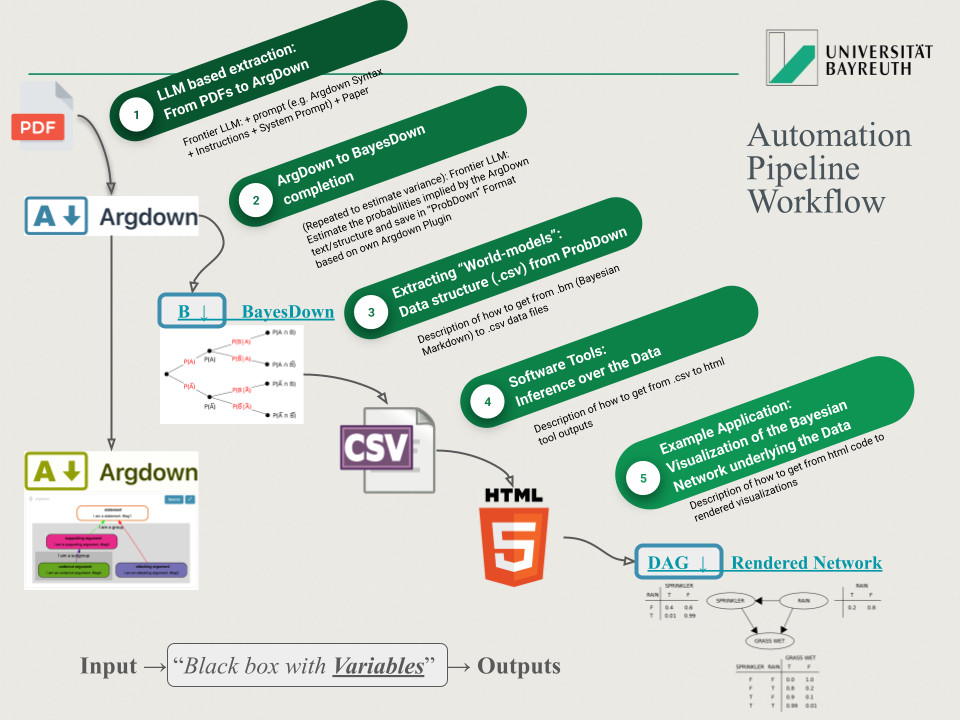
\includegraphics[width=1\linewidth,height=\textheight,keepaspectratio]{images/pipeline.png}}

}

\caption[Five-step AMTAIR automation pipeline from PDFs to Bayesian
networks]{\label{fig-automation_pipeline}AMTAIR Automation Pipeline from
CITATION}

\end{figure}%

Testing crossreferencing grapics Figure~\ref{fig-automation_pipeline}.

\bookmarksetup{startatroot}

\chapter*{Frontmatter}\label{frontmatter}
\addcontentsline{toc}{chapter}{Frontmatter}

\markboth{Frontmatter}{Frontmatter}

\subsection*{\texorpdfstring{\textbf{Acknowledgments}}{Acknowledgments}}\label{acknowledgments}
\addcontentsline{toc}{subsection}{\textbf{Acknowledgments}}

\begin{itemize}
\tightlist
\item
  Academic supervisor (Prof.~Timo Speith) and institution (University of
  Bayreuth)\\
\item
  Research collaborators, especially those connected to the original
  MTAIR project\\
\item
  Technical advisors who provided feedback on implementation aspects\\
\item
  Funding sources and those who provided computational resources or API
  access\\
\item
  Personal supporters who enabled the research through encouragement and
  feedback
\end{itemize}

\bookmarksetup{startatroot}

\chapter*{Prefatory Apparatus: Illustrations and Terminology --- Quick
References}\label{prefatory-apparatus-illustrations-and-terminology-quick-references}
\addcontentsline{toc}{chapter}{Prefatory Apparatus: Illustrations and
Terminology --- Quick References}

\markboth{Prefatory Apparatus: Illustrations and Terminology --- Quick
References}{Prefatory Apparatus: Illustrations and Terminology --- Quick
References}

\section*{List of Tables}\label{list-of-tables}
\addcontentsline{toc}{section}{List of Tables}

\markright{List of Tables}

Table 1: Table name

Table 2: Table name

Table 3: Table name

\begin{itemize}
\tightlist
\item
  Figure 1.1: The coordination crisis in AI governance - visualization
  of fragmentation\\
\item
  Figure 2.1: The Carlsmith model - DAG representation\\
\item
  Figure 3.1: Research design overview - workflow diagram\\
\item
  Figure 3.2: From natural language to BayesDown - transformation
  process\\
\item
  Figure 4.1: ARPA system architecture - component diagram\\
\item
  Figure 4.2: Visualization of Rain-Sprinkler-Grass\_Wet Bayesian
  network - screenshot\\
\item
  Figure 5.1: Extraction quality metrics - comparative chart\\
\item
  Figure 5.2: Comparative analysis of AI governance worldviews - network
  visualization\\
\item
  Table 2.1: Comparison of approaches to AI risk modeling\\
\item
  Table 3.1: Probabilistic translation guide for qualitative
  expressions\\
\item
  Table 4.1: System component responsibilities and interactions\\
\item
  Table 5.1: Policy impact evaluation results - summary metrics
\end{itemize}

\section*{List of Graphics \& Figures}\label{list-of-graphics-figures}
\addcontentsline{toc}{section}{List of Graphics \& Figures}

\markright{List of Graphics \& Figures}

\section*{List of Abbreviations}\label{list-of-abbreviations}
\addcontentsline{toc}{section}{List of Abbreviations}

\markright{List of Abbreviations}

esp.~especially

f., ff.~following

incl.~including

p., pp.~page(s)

MAD Mutually Assured Destruction

\begin{itemize}
\tightlist
\item
  AI - Artificial Intelligence\\
\item
  AGI - Artificial General Intelligence\\
\item
  ARPA - AI Risk Pathway Analyzer\\
\item
  DAG - Directed Acyclic Graph\\
\item
  LLM - Large Language Model\\
\item
  MTAIR - Modeling Transformative AI Risks\\
\item
  P(Doom) - Probability of existential catastrophe from misaligned AI\\
\item
  CPT - Conditional Probability Table
\end{itemize}

\section*{Glossary}\label{glossary}

\markright{Glossary}

\begin{itemize}
\tightlist
\item
  \textbf{Argument mapping}: A method for visually representing the
  structure of arguments\\
\item
  \textbf{BayesDown}: An extension of ArgDown that incorporates
  probabilistic information\\
\item
  \textbf{Bayesian network}: A probabilistic graphical model
  representing variables and their dependencies\\
\item
  \textbf{Conditional probability}: The probability of an event given
  that another event has occurred\\
\item
  \textbf{Directed Acyclic Graph (DAG)}: A graph with directed edges and
  no cycles\\
\item
  \textbf{Existential risk}: Risk of permanent curtailment of humanity's
  potential\\
\item
  \textbf{Power-seeking AI}: AI systems with instrumental incentives to
  acquire resources and power\\
\item
  \textbf{Prediction market}: A market where participants trade
  contracts that resolve based on future events\\
\item
  \textbf{d-separation}: A criterion for identifying conditional
  independence relationships in Bayesian networks\\
\item
  \textbf{Monte Carlo sampling}: A computational technique using random
  sampling to obtain numerical results
\end{itemize}

\section*{\texorpdfstring{Checklists }{Checklists }}\label{checklists}
\addcontentsline{toc}{section}{Checklists }

\markright{Checklists }

\section*{``Usual paper requirements''}\label{usual-paper-requirements}
\addcontentsline{toc}{section}{``Usual paper requirements''}

\markright{``Usual paper requirements''}

\begin{itemize}
\tightlist
\item
  introduce all terminology

  \begin{itemize}
  \tightlist
  \item
    go through text, make sure all terms are defined, explained (and
    added to the list of Abbr.) when first mentioned\\
  \end{itemize}
\item
  readership is intelligent and interested but has no prior knowledge
\end{itemize}

\section*{}\label{section}
\addcontentsline{toc}{section}{}

\markright{}

\section*{(Format:) \textasciitilde{} Anything that makes it easier to
understand}\label{format-anything-that-makes-it-easier-to-understand}
\addcontentsline{toc}{section}{(Format:) \textasciitilde{} Anything that
makes it easier to understand}

\markright{(Format:) \textasciitilde{} Anything that makes it easier to
understand}

\begin{itemize}
\tightlist
\item
  short sentences\\
\item
  paragraphs (one idea per paragraph)\\
\item
  simplicity\\
\item
  !limit use of passive voice!\\
\item
  use active voice, even prefer I over we!\\
\item
  minimise use of ``zombi nouns'' (don't turn verbs/adjectives to
  nouns!)\\
\item
  ``find words that can be cut''
\end{itemize}

-- the paper can \textbf{focus} on \textbf{one aspect of the
presentation}

-- ``open door policy'' for (content) questions

\textasciitilde{} demonstrate ability for novel research

-- ``solve research question with the tools accessible to you''

-- ``show something that has not been shown before / should be
publishable in principle''

-- new idea (or criticism) ``in this field''

-- Outline idea THEN reading with a purpose (answering concrete
questions)

-- ``Only'' confirm that nobody has published the exact same idea on the
same topic

-- pretty much determined by presentation \& proposal but narrow down
further (\& choose supervisor?)

\subsection*{Quarto Features Incompatible with LaTeX
(Below)}\label{quarto-features-incompatible-with-latex-below}

\bookmarksetup{startatroot}

\chapter{Quarto Syntax}\label{quarto-syntax}

\section*{Figures}\label{sec-figues}

\markright{Figures}

\begin{figure}

\centering{

\href{https://github.com/VJMeyer/submission}{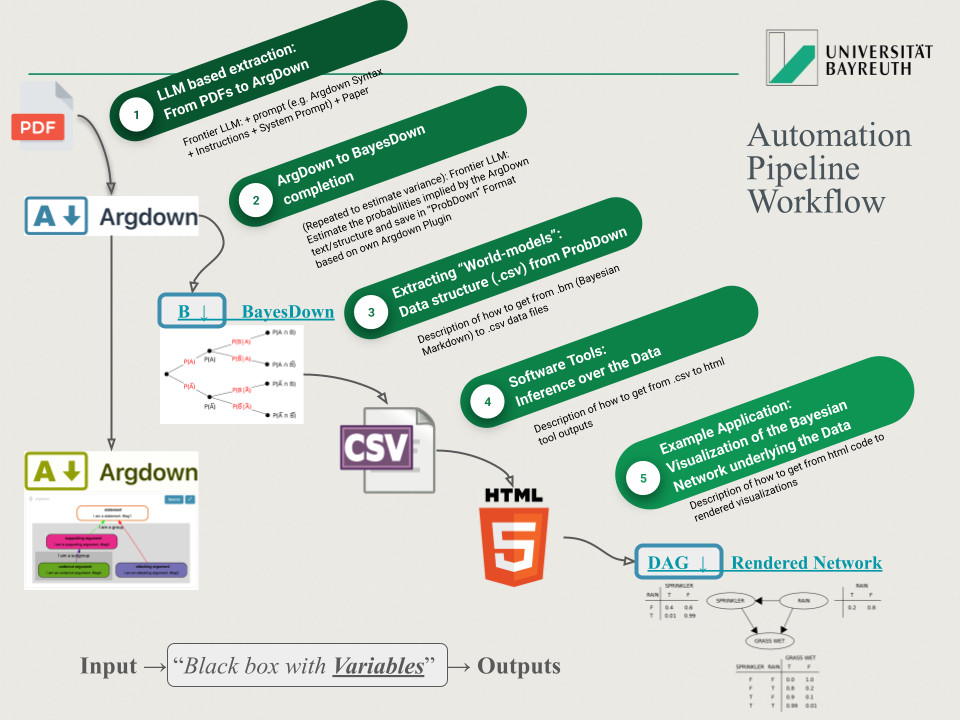
\includegraphics[width=1\linewidth,height=\textheight,keepaspectratio]{images/pipeline.png}}

}

\caption[Five-step AMTAIR automation pipeline from PDFs to Bayesian
networks]{\label{fig-automation_pipeline}AMTAIR Automation Pipeline from
\textcite{bucknall2022}}

\end{figure}%

Testing crossreferencing grapics Figure~\ref{fig-automation_pipeline}.

\begin{figure}


\includegraphics[width=0.3\linewidth,height=\textheight,keepaspectratio]{images/cover.png}

\caption[Short 2 caption]{\label{fig-testgraphic2}Caption/Title 2}

\end{figure}%

Testing crossreferencing grapics Figure~\ref{fig-testgraphic2}.

\section*{Citations}\label{sec-citations}

\markright{Citations}

\textcite{soares2014}

\autocite{soares2014} and \autocite{knuth1984}

Blah Blah \autocites[see][33-35]{knuth1984}[also][chap.~1]{growiec2024}

Blah Blah \autocite[33-35, 38-39 and passim]{knuth1984}

Blah Blah \autocite{growiec2024,knuth1984}.

Growiec says blah \autocite*{growiec2024}

\section{Headings \& Potential Headings}\label{sec-heading}

\texttt{verbatim\ code\ formatting\ for\ notes\ and\ ideas\ to\ be\ included\ (here)}

\begin{verbatim}
Also code blocks for more extensive notes and ideas to be included and checklists
- test 1. 
- test 2. 
- test 3.
2. second
3. third
\end{verbatim}

\begin{quote}
Blockquote formatting for ``Suggested Citations (e.g.~carlsmith 2024 on
\ldots)'' and/or claims which require a citation (e.g.~claim x should be
backed-up by a ciation from the literature)
\end{quote}

Here is an inline note.\footnote{Inlines notes are easier to write,
  since you don't have to pick an identifier and move down to type the
  note.}

Here is a footnote reference,\footnote{Here is the footnote.}

\renewcommand*{\labelitemi}{\textgreater}

Here's some raw inline HTML:

page 1

\newpage{}

page 2

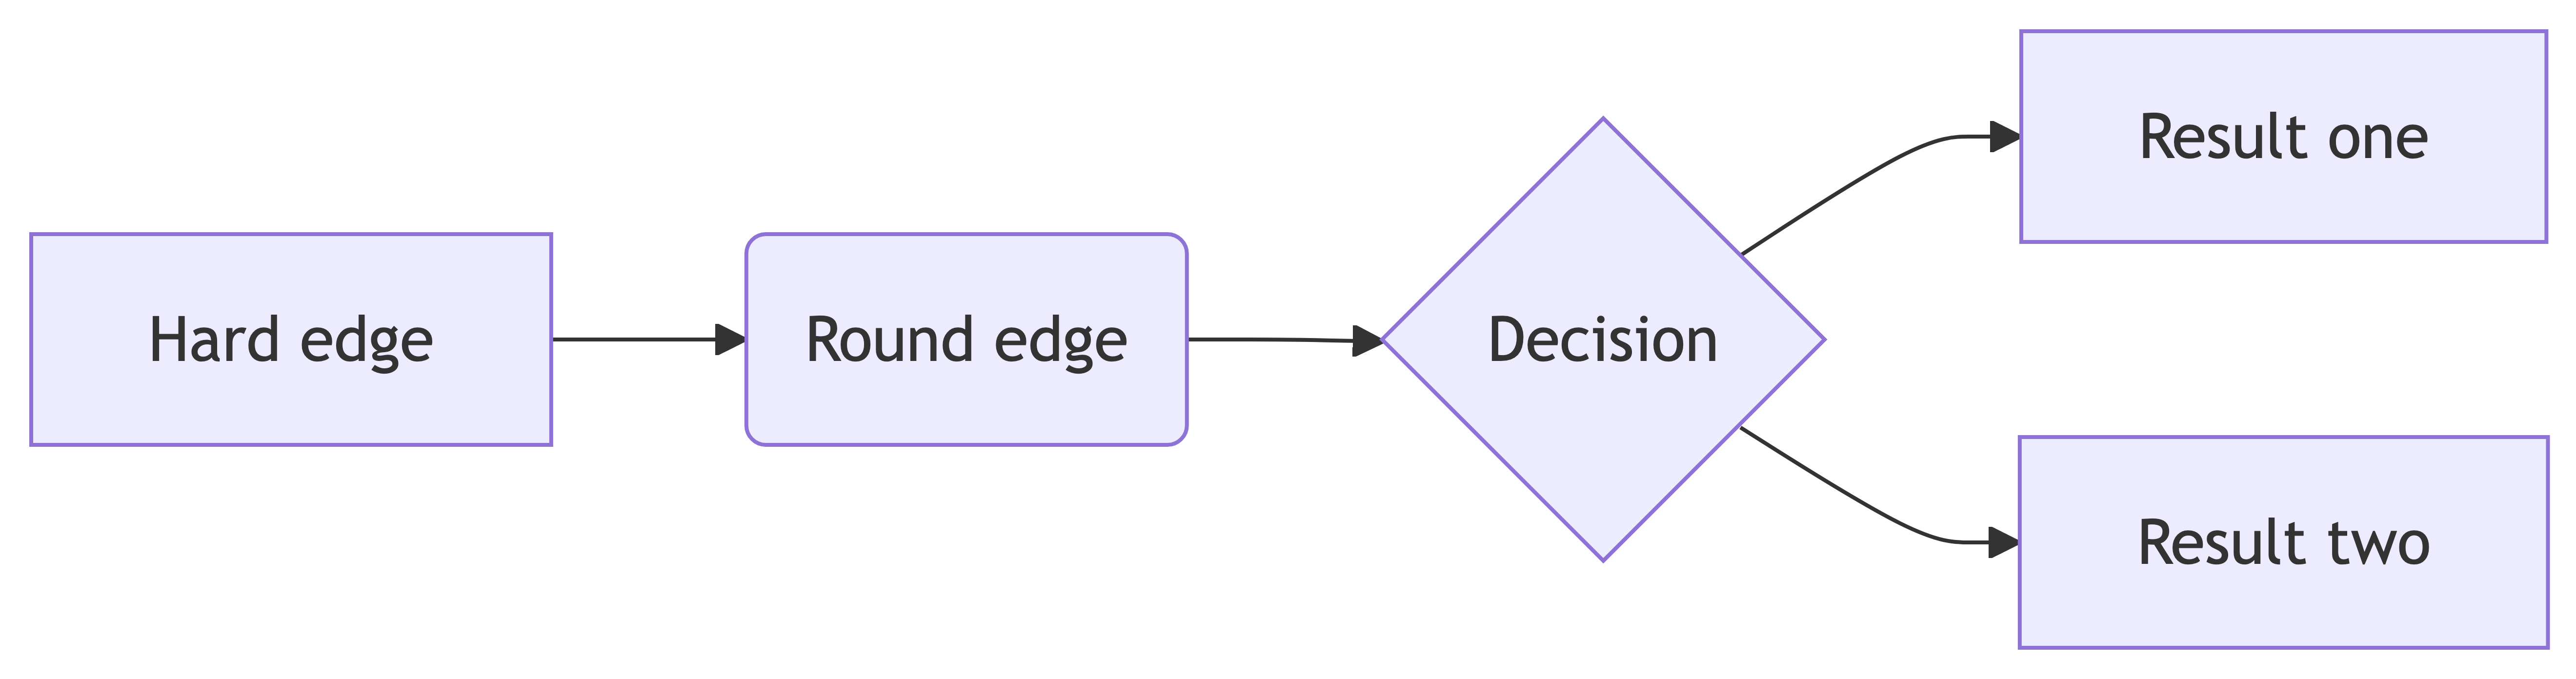
\includegraphics[width=6.88in,height=1.81in]{ref/references_files/figure-latex/mermaid-figure-1.png}

Testing crossreferencing grapics Figure~\ref{fig-automation_pipeline}.

\bookmarksetup{startatroot}

\chapter*{Bibliography (References)}\label{bibliography-references}
\addcontentsline{toc}{chapter}{Bibliography (References)}

\markboth{Bibliography (References)}{Bibliography (References)}


% % Add affidavit at the end but still within document environment
% % \pagenumbering{Roman} % Switch to Roman page numbering
% 
\clearpage
\thispagestyle{empty} % Removes page numbering for current page

\newpage


% Top header with logo (left) and department (right)
\begin{minipage}{0.3\textwidth}
  
\includegraphics[width=5cm]{latex/uni-bayreuth-logo.png}
\end{minipage}
\hfill
\begin{minipage}{0.9\textwidth}
  \begin{center}
    -- P\&E Master's Programme --\\
    Chair of Philosophy, Computer\\
    Science \& Artificial Intelligence
  \end{center}
\end{minipage}

% Horizontal rule
\vspace{1.5cm}
\hrule
\vspace{2.5cm}

% Title in bold

  \LARGE\textbf{Affidavit}
\vspace{1.5cm}

\center

\normalsize

% \part*{Affidavit}

    \subsection*{\Large Declaration of Academic Honesty}
	    \vspace{1cm}\noindent \\
	    Hereby, I attest that I have composed and written the presented thesis 
        \vspace*{0.5cm}\noindent \\
        \textit{ \textbf{ Automating the Modelling of Transformative Artificial Intelligence Risks }}
        \vspace*{0.5cm}\noindent \\
        independently on my own, without the use of other than the stated aids and without any other resources than the ones indicated. All thoughts taken directly or indirectly from external sources are properly denoted as such.
	    \vspace{\baselineskip}
	    \\  This paper has neither been previously submitted in the same or a similar form to another authority nor has it been published yet.
	    \vspace{2cm}
	    
    \flushright
    \begin{minipage}{0.5\textwidth}
        \begin{flushleft} \large
        \textsc{Bayreuth}                     %   Place
        on the \\ % 26th of May 2025     \\
        \today           %   Date
        \vspace{2cm}\\
    	{\rule[-3pt]{\linewidth}{.4pt}\par\smallskip  
        \textsc{Valentin Meyer}	\\         %   Your name
    	}
        \end{flushleft}
        \end{minipage}


% \end{document}

















% % After loading packages but before \begin{document}
% \AtBeginDocument{
%   % Set up page styles
%   \fancypagestyle{frontmatter}{
%     \fancyhf{}
%     \fancyfoot[C]{\thepage}
%     \renewcommand{\footrulewidth}{0pt}
%   }

%   \fancypagestyle{mainmatter}{
%     \fancyhf{}
%     \fancyhead[LE,RO]{\slshape\nouppercase{\rightmark}}
%     \fancyhead[LO,RE]{\slshape\nouppercase{\leftmark}}
%     \fancyfoot[C]{\thepage}
%   }
% }

% % Inside the document, after title page
% \frontmatter
% \pagestyle{frontmatter}

% % Added automatically before Introduction
% % \mainmatter
% % \pagestyle{mainmatter}
